%%%%%%%% ICML 2026 EXAMPLE LATEX SUBMISSION FILE %%%%%%%%%%%%%%%%%

\documentclass{article}
\input{math_commands.tex}
% Recommended, but optional, packages for figures and better typesetting:
\usepackage{microtype}
\usepackage{graphicx}
\usepackage{subcaption}
\usepackage{booktabs} % for professional tables

% hyperref makes hyperlinks in the resulting PDF.
% If your build breaks (sometimes temporarily if a hyperlink spans a page)
% please comment out the following usepackage line and replace
% \usepackage{icml2026} with \usepackage[nohyperref]{icml2026} above.
\usepackage{hyperref}
\usepackage{makecell}


% Attempt to make hyperref and algorithmic work together better:
\newcommand{\theHalgorithm}{\arabic{algorithm}}

% Use the following line for the initial blind version submitted for review:
%\usepackage{icml2026}
\usepackage{icml2026}

% For preprint, use
% \usepackage{icml2026}

% If accepted, instead use the following line for the camera-ready submission:
% \usepackage{icml2026}

\usepackage{amsmath}
\usepackage{amssymb}
\usepackage{mathtools}
\usepackage{amsthm}
\usepackage{algorithm}
\usepackage{algorithmic}

% Color package for highlighting new additions
\usepackage{xcolor}
\definecolor{newaddition}{rgb}{0.0,0.4,0.7}
\newcommand{\newnew}[1]{\begingroup\color{newaddition}#1\endgroup}
\newcommand{\RETURN}{\STATE \textbf{return }}
\newcommand{\ram}[1] {\textcolor{purple}{[RM. #1]}}
\newcommand{\jh}[1] {\textcolor{cyan}{[JH. #1]}}

% if you use cleveref..
\usepackage[capitalize,noabbrev]{cleveref}

%%%%%%%%%%%%%%%%%%%%%%%%%%%%%%%%
% THEOREMS
%%%%%%%%%%%%%%%%%%%%%%%%%%%%%%%%
\theoremstyle{plain}
\newtheorem{theorem}{Theorem}[section]
\newtheorem{proposition}[theorem]{Proposition}
\newtheorem{lemma}[theorem]{Lemma}
\newtheorem{corollary}[theorem]{Corollary}
\theoremstyle{definition}
\newtheorem{definition}[theorem]{Definition}
\newtheorem{assumption}[theorem]{Assumption}
\theoremstyle{remark}
\newtheorem{remark}[theorem]{Remark}

% Todonotes is useful during development; simply uncomment the next line
%    and comment out the line below the next line to turn off comments
%\usepackage[disable,textsize=tiny]{todonotes}
\usepackage[textsize=tiny]{todonotes}

% The \icmltitle you define below is probably too long as a header.
% Therefore, a short form for the running title is supplied here:
\icmltitlerunning{Test-time Generalization for Physics through Neural Operator Splitting}

\begin{document}

\twocolumn[
  \icmltitle{Test-time Generalization for Physics through Neural Operator Splitting}
  
  \icmlsetsymbol{visiting}{*}
   \icmlsetsymbol{corresponding}{\dag}
  
  \begin{icmlauthorlist}\icmlauthor{Anonymous}{anon}\end{icmlauthorlist}

   \vskip 0.1in
  \centerline{\textbf{The Polymathic AI Collaboration}}
  \vskip 0.1in
  
  
  % \icmlaffiliation{anon}{Anonymous Institution}
  
  
  
  
  

  %\icmlauthornote{corresponding}{Corresponding author.}
  \icmlcorrespondingauthor{Anonymous}{anonymous@anonymous.invalid}
  
  \icmlkeywords{Machine Learning, PDE, Neural Surrogates, Test-Time, ICML}
  \vskip 0.3in
]
% This must go AFTER the closing bracket ]

% this must go after the closing bracket ] following \twocolumn[ ...

% This command actually creates the footnote in the first column listing the
% affiliations and the copyright notice. The command takes one argument, which
% is text to display at the start of the footnote. The \icmlEqualContribution
% command is standard text for equal contribution. Remove it (just {}) if you
% do not need this facility.

% Use ONE of the following lines. DO NOT remove the command.
% If you have no special notice, KEEP empty braces:
\printAffiliationsAndNotice{%
    %\textsuperscript{*}Work conducted during an internship at Polymathic AI. %
    \textsuperscript{\dag}Corresponding author.%
} % no special notice (required even if empty)
% Or, if applicable, use the standard equal contribution text:
% \printAffiliationsAndNotice{\icmlEqualContribution}

\begin{abstract}
 
Neural operators have shown promise in learning solution maps of partial differential equations (PDEs), but they often struggle to generalize when test inputs lie outside the training distribution, such as novel initial conditions, unseen PDE coefficients or unseen physics. Prior works address this limitation with large-scale multiple physics pretraining followed by fine-tuning, but this still requires examples from the new dynamics, falling short of true zero-shot generalization. 
In this work, we propose a method to enhance generalization at test time, i.e., without modifying pretrained weights. Building on DISCO, which provides a dictionary of neural operators trained across different dynamics, we introduce a neural operator splitting strategy that, at test time, searches over compositions of training operators to approximate unseen dynamics.
On challenging out-of-distribution tasks including parameter extrapolation and novel combinations of physics phenomena, our approach achieves state-of-the-art zero-shot generalization results, while being able to recover the underlying PDE parameters. 
These results underscore test-time computation as a key avenue for building flexible, compositional, and generalizable neural operators.
\end{abstract}

\section{Introduction}

Neural surrogates \citep{bezenac2017,han2021machine, pfaff2020learning,Brandstetter2022} and neural operators \citep{Lu2019, li2020fourier, Kovachki2022, raonic2023convolutional, serrano2023coral, boulle2024operator} offer powerful data-driven tools for modeling spatiotemporal dynamics and systems governed by partial differential equations (PDEs). 
Their main limitation, however, is 
% vulnerability
sensitivity 
to distribution shifts at test time, i.e., when the dynamics are out-of-distribution (OOD). Such shifts can arise from variations in initial conditions \citep{chen2024data}, error accumulation during autoregressive rollouts \citep{Brandstetter2022, Lippe2023, pedersen2025thermalizer}, changes in PDE parameters \citep{kirchmeyer2022generalizing, koupai2024geps}, or fundamentally different underlying dynamics \citep{takamoto2022pdebench, mccabe2023multiple, herde2024poseidon}.

We focus on the \emph{parametric setting} \citep{approximationpdes}, where a neural surrogate is trained to emulate families of physical dynamics indexed by multi-dimensional coefficient vectors, often corresponding to distinct physical effects. Beyond interpolation within a fixed parameter regime, we are interested in assessing the ability of such surrogates to extrapolate, either to parameter configurations never encountered during training or to novel combinations of physical effects observed only in isolation, while having access to only limited observation data for test-time adaptation.

% To address failures under OOD conditions, 
To address failures in OOD settings, 
many recent frameworks \citep{mccabe2023multiple, herde2024poseidon, hao2024dpot} adopt a \emph{pretrain–then–finetune} paradigm. While often effective, this strategy breaks down when very limited data are available for fine-tuning \citep{koupai2024geps}, and the models face fundamental limitations due to their lack of compositionality, with generalization effectively limited to the span of dynamics represented in the pretraining distribution.

Meta-learning~\citep{thrun1998learning,finn2017modelagnostic} offers an alternative, aiming to learn shared representations that can be rapidly adapted to new parameter regimes \citep{yin2022leads, kirchmeyer2022generalizing, koupai2024geps, nzoyem2025neural}. However, these approaches have yet to scale reliably to diverse physical systems \citep{ohana2024well, morel2025disco}, and parameter adaptation has been shown to be unstable under 
% OOD
distribution 
shifts \citep{serrano2025zebra}.

% To overcome these limitations, we propose a novel test-time adaptation approach for neural surrogates that increases expressivity and predictive quality while keeping model weights fixed. Our method approximates unobserved dynamics as a sum of neural operators learned during training.
To overcome these limitations, we propose a novel test-time adaptation approach based on neural operator splitting. Without modifying the weights of our model, our method approximates test-time dynamics as compositions of operators learned during training, enabling generalization beyond the set of physical phenomena seen during training.
The framework consists of three components: 
(1) a pretrained DISCO model~\citep{morel2025disco}, a scalable framework that infers a neural operator from each training trajectory and encodes it in a shared, compact latent space;
(2) an efficient test-time beam search over the discrete operators discovered during training to identify a suitable decomposition of the unknown dynamics; 
and (3) operator splitting \citep{Strang1968OnTC}, used both during the search and rollout to approximate the sum of physical terms through successive compositions.
% This test-time strategy comes at a higher computational cost, but enables better adaptation when faced with unseen dynamics. \jh{Soften this claim a bit according to Slack discussion? perhaps also add related comments in the method part}
Beyond improved test-time adaptation, our method enables system identification by expressing unknown dynamics as compositions of known training operators and is naturally adaptive, requiring less search near the training distribution and more extensive search in far OOD settings.

We evaluate our method against existing approaches on two challenging OOD zero-shot scenarios: when the PDE coefficients lie outside the training distribution, and when the spatiotemporal dynamics result from combinations of physical processes that were observed only individually during training.
Our results show that the proposed approach outperforms other methods in both zero-shot settings. 
Our key contributions are as follows:

\begin{itemize}
\item We propose a novel test-time generalization strategy for evolving PDEs 
based on neural operator splitting
% that combines neural operators with operator splitting 
to approximate OOD spatiotemporal dynamics.
\item We adapt a beam search procedure to combine pretrained operators, balancing accuracy and compute, and provide corresponding test-time scaling laws.
% \item We demonstrate state-of-the-art zero-shot generalization across diverse nonlinear PDEs and tasks, including parameter extrapolation and operator composition—outperforming adaptive neural operator methods and transformer, based architectures.
\item We demonstrate state-of-the-art zero-shot generalization across diverse nonlinear PDEs on tasks such as parameter extrapolation and operator composition, outperforming adaptive neural operator methods and transformer-based architectures.
% \item Analysis of the resulting operator decompositions reveals unseen dynamics and enables zero-shot PDE parameter estimation.
\item Analysis of the resulting operator decompositions enables system identification and zero-shot PDE parameter estimation.
\item To the best of our knowledge, this is the first work to tackle test-time generalization with fixed model weights for predicting PDEs.
\end{itemize}


\begin{figure*}[t]
\centering
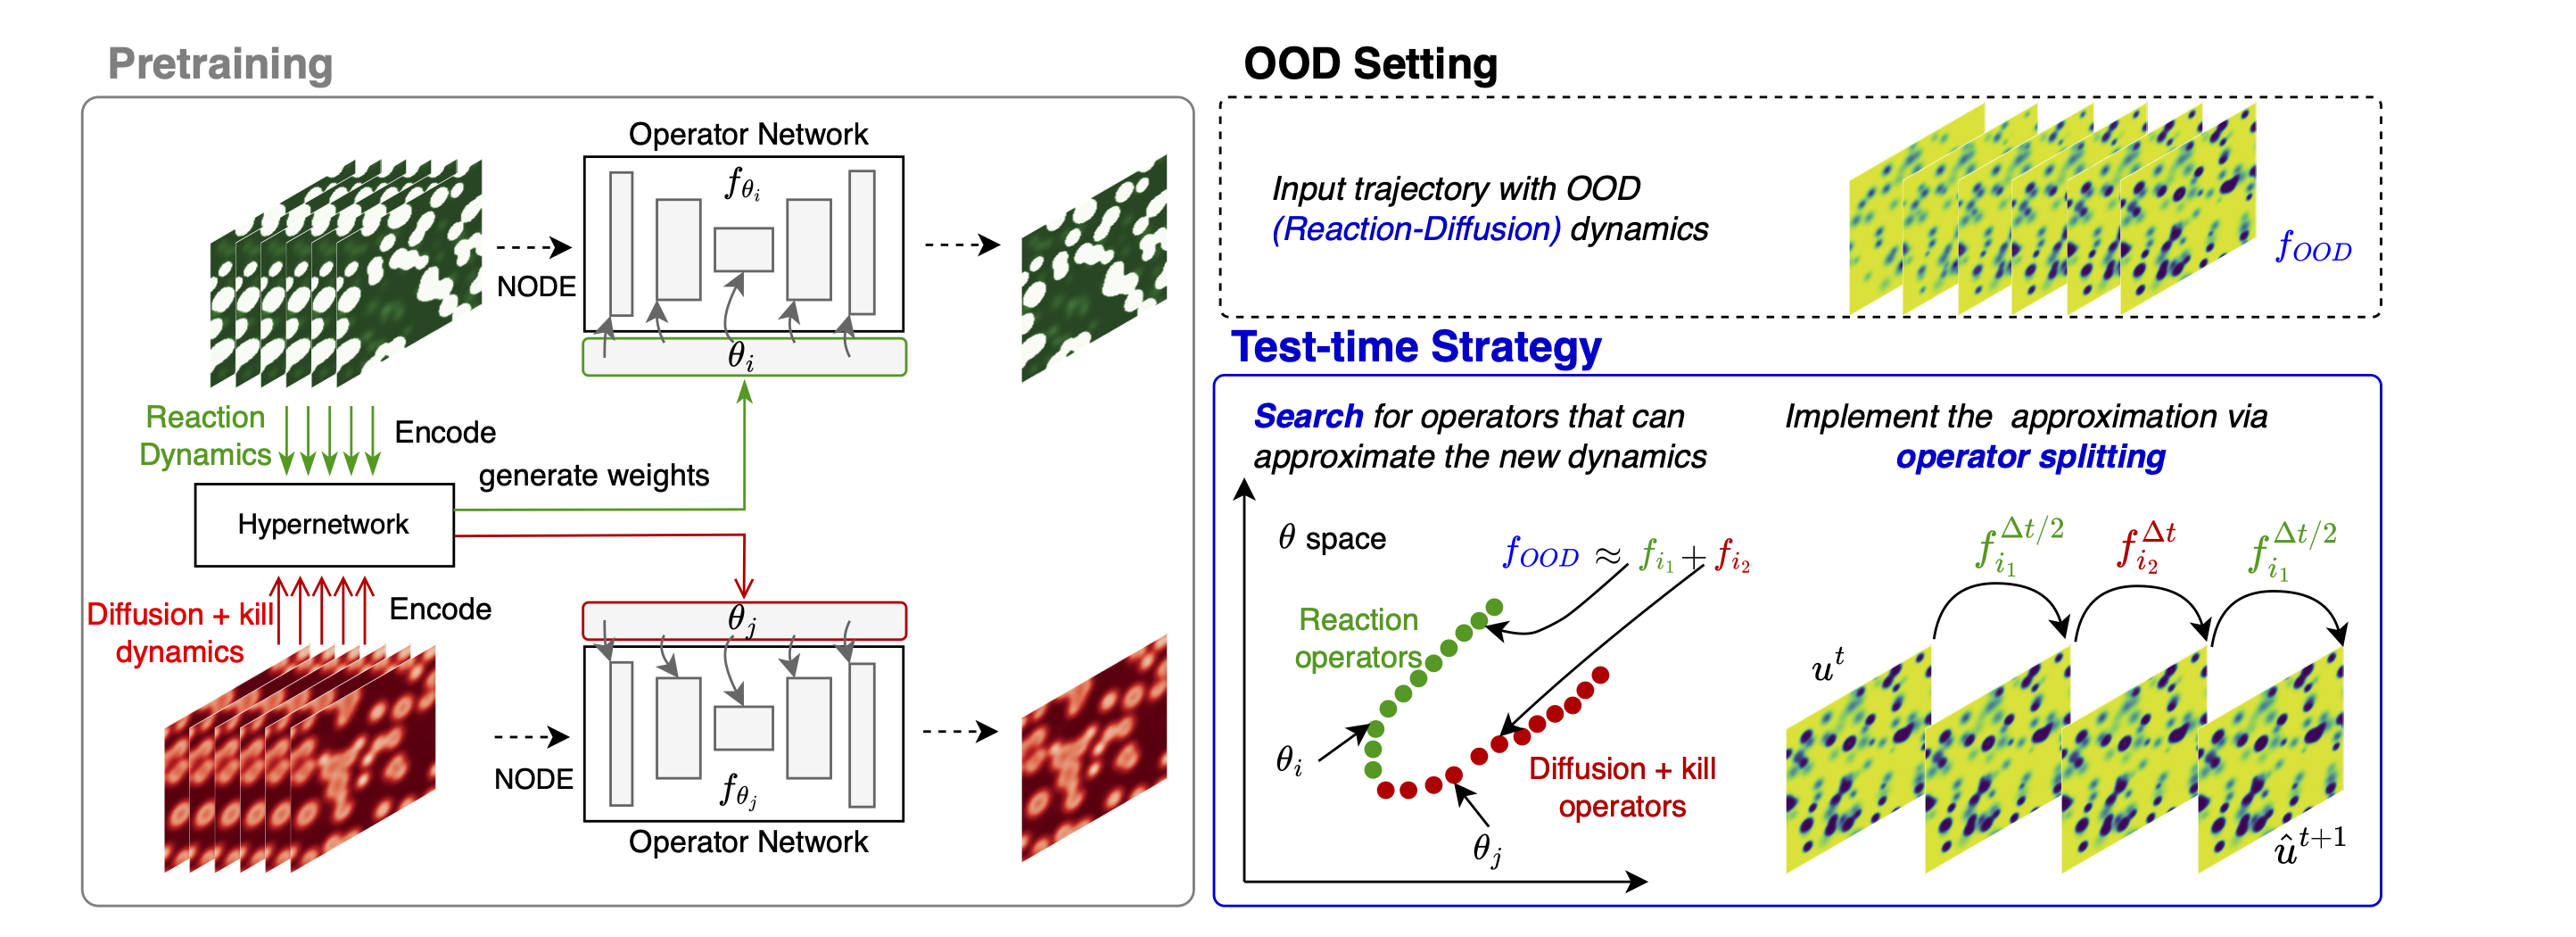
\includegraphics[width=\textwidth]{figures/main_figure_arxiv.png}
\caption{
\textbf{Test-time generalization through neural operator splitting}.
During pretraining (left), DISCO learns a dictionary of operators for different physics, such as reaction dynamics (green) and diffusion+kill dynamics (red), with a hypernetwork generating corresponding operator weights $\theta_i, \theta_j$.
At test time (right), on OOD dynamics such as reaction-diffusion, our method searches over combinations of these operators to approximate the new dynamics (e.g., $f_{OOD} \approx f_{i_1} + f_{i_2}$), and evolves $u^t \rightarrow u^{t+1}$ using neural operator splitting via sequential operator applications. 
%\jh{Refer to Figure 1 somewhere}
}
\label{fig:method_placeholder}
\end{figure*}


\section{Related Work}


\paragraph{Neural surrogate models and out-of-distribution generalization.}
Neural surrogate models have emerged as a powerful tool for accelerating simulation-based workflows for partial differential equations, enabled by the availability of large benchmark datasets and advances in neural operator architectures~\citep{takamoto2022pdebench,ohana2024well,koehler2024apebench,mccabe2023multiple,hao2024dpot, morel2025disco}. When trained at scale, these models can achieve high accuracy on in-distribution tasks. However, their performance often degrades sharply when used in out-of-distribution settings, such as unseen PDE parameters, forcing terms, or compositions of physical effects. 
A response to this challenge is to further scale pretraining by increasing datasets, model and compute size, followed by fine-tuning on OOD target data~\citep{herde2024poseidon, NCWNO, mccabe2025walrus}.
This paradigm implicitly assumes access to enough OOD target samples, which may be unavailable or expensive to obtain in practice.

% Our method proposes a different direction by focusing on 
% A dominant response to this challenge has been to further scale pretraining datasets and model capacity, followed by fine-tuning on OOD target data~\citep{herde2024poseidon, NCWNO, mccabe2025walrus}. 
% \ram{Mention the fact that fine-tuning blindly doesn't }
% While effective, this paradigm implicitly assumes access to at least a small number of samples from the target system at deployment, which may be unavailable or expensive to obtain in practice.

% \paragraph{Sample-efficient adaptation and meta-learning for dynamical systems.}
\paragraph{Meta-learning for dynamical systems.}
To reduce reliance on extensive target data, a second line of work focuses on sample-efficient adaptation through meta-learning. 
% or structured generalization across tasks. 
These methods aim to rapidly adapt to new PDEs by exploiting shared structure, but often rely on strong assumptions, such as known PDE coefficients~\citep{wang2022meta}, symmetry information~\citep{mialon2023self}, or restrictive parameterizations~\citep{blanke2023interpretable}. CODA ~\citep{kirchmeyer2022generalizing} and GEPS \citep{koupai2024geps} relax some of these constraints by adapting a shared neural operator to unseen physics, but still requires gradient-based fine-tuning at test time, which can be computationally expensive, especially in far OOD regimes.
In contrast, in this paper we design a method that operates at test time without fine-tuning a base model, instead relying on search. Specifically, our method uses the pretrained model to search for an operator that best fits a potentially single target trajectory, without relying on explicit knowledge of the governing equations at test time.
% that does not require fine-tuning a base model, without explicit knowledge of the governing equations at test time. 
% In contrast, in this paper we delibarately design a method that .. curcircuits adaptation of the parameters of the model. 
% DISCO~\citep{morel2025disco} takes a complementary approach by encoding training trajectories into a latent space of neural operators, enabling generalization to complex and unseen physics without explicit knowledge of governing equations.

\paragraph{In-context learning and compositional generalization.}
More recently, several works have explored in-context learning and compositional mechanisms for differential equations. ICON~\citep{icon} demonstrates in-context prediction for ODEs by conditioning on example trajectories of related systems, enabling adaptation without parameter updates. \citet{Cao2024, serrano2025zebra, koupai2025enma} extend this idea to PDEs, showing that models can in some cases generalize in context by conditioning on solutions from related tasks. However, the mechanisms by which they implicitly compose or reuse physical operators often remain implicit and difficult to access. 
For example, recent work by ~\citet{fear2025physics} rely on identifying hidden steering vectors tied to specific physical phenomena, requiring careful post hoc probing of model activations. 
In our paper, we instead rely on the explicit composition of neural operators in order to provide an adaptation strategy to OOD settings without requiring training on target data. 
Our method searches over compositions of pretrained operators identified during training by DISCO~\cite{morel2025disco} and selects the one that best fits an observation of the OOD target trajectory. To our knowledge, this is the first work to bring search-based adaptation and test-time compute scaling to neural PDE solvers.

% \paragraph{Test-time computation and operator composition.} In parallel, the large language model literature has shown that substantial gains can be achieved by reallocating computation to test time, using strategies such as Best-of-$N$ sampling and beam search to explore multiple candidate solutions without modifying model parameters~\citep{huang2025best,xie2023self,meta2025llama4,mistral2025medium3,openai2025gpt5}. Inspired by these developments, we introduce a test-time adaptation strategy for PDEs that exploits the compositional structure of neural operators learned by DISCO \cite{morel2025disco}. Rather than fine-tuning or conditioning on external demonstrations, our method explicitly searches over compositions of pretrained operators and selects the one that best explains a short observation window from the target trajectory. This shifts adaptation entirely to test time, requires no target training data, and leverages classical operator splitting to provide a principled mechanism for compositional generalization. To our knowledge, this is the first work to bring test-time compute scaling and search-based adaptation to neural PDE solvers.


%\paragraph{Surrogate models for PDEs.}
%With the goal of accelerating simulation-based workflows, and supported by growing collections of datasets~\citep{takamoto2022pdebench,ohana2024well,koehler2024apebench}, surrogate models~\citep{mccabe2023multiple,hao2024dpot,herde2024poseidon,serrano2025zebra,morel2025disco} have gradually improved their pretraining performance, and achieve better results than training from scratch when fine-tuned on out-of-distribution PDEs.
%In contrast, our approach operates at test time without updating the model weights.

%\paragraph{Meta-learning strategies for dynamical systems.}
%\paragraph{Adaptation for dynamical systems.}
%Meta-learning strategies aim at rapidly adapting to new tasks (e.g., unseen PDE coefficients) by leveraging shared weights across tasks. However, many methods make restrictive assumptions, such as knowing the new PDE coefficients~\citep{wang2022meta}, PDE symmetries~\citep{mialon2023self}, or affine predictability~\citep{blanke2023interpretable}. 
%In GEPS, \citet{kirchmeyer2022generalizing,koupai2024geps} adapt a shared operator to unseen physics, but this still requires fine-tuning a neural operator, which can be costly, especially in far OOD scenarios.
%In contrast, our approach builds on DISCO~\citep{morel2025disco}, which encodes the training set into a latent space of neural operators from the trajectory data only, and can generalize to unseen complex physics phenomena and PDE parameters well beyond the training range.

%\newnew{\paragraph{In-context learning and operator composition for PDEs.}
%Several recent works explore compositional and in-context learning approaches for PDE solving. ICON~\citep{grigas2024context} introduces in-context operator networks that learn to predict ODE solutions by conditioning on demonstrations of similar systems, operating in a fundamentally different regime where the model learns from examples of complete solution trajectories rather than learning operators from individual physics components. NCWNO~\citep{pan2024learning} proposes a continual learning framework where previously learned solutions guide adaptation to new PDEs, requiring access to training data from related tasks and performing sequential weight updates. Poseidon~\citep{herde2024poseidon} develops a multi-physics foundation model that adapts through fine-tuning with limited observations, typically requiring at least a single full trajectory snapshot from the target dynamics. While these approaches demonstrate promising compositional capabilities, they operate in settings distinct from our zero-shot test-time regime: ICON focuses on ODE in-context prediction rather than PDE operator composition, NCWNO requires continual access to training data during adaptation, and Poseidon relies on weight fine-tuning with target examples. In contrast, our method performs zero-shot adaptation by composing pretrained operators through classical splitting schemes, without any weight updates or access to target training data, instead relying solely on a short observation window from the test trajectory.}

%\paragraph{Test-time strategies.}
%Methods to improve model performance at test time (i.e., after pretraining) have emerged with the scaling of large language models~\citep{meta2025llama4,mistral2025medium3,openai2025gpt5}. In Best-of-N, the model generates multiple candidate outputs and selects the best one according to a predefined criterion or reward~\citep{huang2025best}. Beam search extends this idea by maintaining and refining a set of promising output sequences as the model generates them~\citep{xie2023self}.
%Similarly, our approach allocates additional compute at test time by exploring different compositions of operators seen during training and selecting the one that best fits the beginning of the test-time trajectory. To our knowledge, this is the first work to introduce test-time strategies for evolving dynamical systems governed by PDEs, and we further provide test-time compute scaling laws~\citep{hestness2017deep} in this context.


\section{Problem Setting}
\label{sec:problem-setting}

Data-driven models for evolving unknown PDEs are typically trained on trajectories with varying PDE class, coefficients, and initial conditions, with the goal of generalizing to unseen scenarios. While prior work has generally emphasized generalization over novel initial conditions under a fixed PDE, we consider the additional challenge of generalizing to unseen PDE coefficients or even entirely new PDE classes. This setting relates to approaches such as MPP~\citep{mccabe2023multiple},  DISCO~\citep{morel2025disco} or WALRUS \citep{mccabe2025walrus}, but we restrict the diversity of training physics to better evaluate OOD generalization.


\paragraph{Parametric PDE setting.} 
We consider a family of parametric PDEs of the form
$$
\partial_t u = \sum_{k=1}^K \mu_k \, \mathcal{F}_k(u, \nabla_x u, \nabla^2_x u, \ldots),
$$
where $u(x,t)$ is the solution field, $\mu = (\mu_1, \ldots, \mu_K) \in \mathcal{M}$ is a parameter vector, and $\{\mathcal{F}_k\}_k$ denote fundamental physics operators (e.g., advection, diffusion, reaction, etc.). During training, parameters are drawn from a \textit{sparse distribution} $P^{\text{train}}(\mu)$, where only one operator is 
% active
present for each trajectory. Concretely, each sample takes the form 
% $\mu = (0, \ldots, 0, \mu_k, 0, \ldots, 0)$,
$\mu = (0, \ldots, \mu_k, \ldots, 0)$,
with exactly one nonzero component $\mu_k \in \mathcal{M}_k^{\text{train}}$, restricted to a prescribed training range.


\paragraph{OOD challenges.} 
This training setup naturally induces two distinct types of OOD 
scenarios at test time:
\begin{itemize}
\item \textit{Parameter Extrapolation}: Parameters remain sparse but take values \textit{outside} the convex hull of training ranges:
$\mu_{\text{test}} = (0, \ldots, \mu_k^{\text{test}}, \ldots, 0)$ 
with $\mu_k^{\text{test}} \notin \text{conv}(\mathcal{M}_k^{\text{train}})$.

\item \textit{Operator Composition}: Multiple operators are simultaneously 
% active, 
present, 
though each parameter still lies \textit{within} its training range:
$\mu_\text{test} = (\mu_1, \ldots, \mu_K)$ with several $\mu_k \neq 0$ and $\mu_k \in \text{conv}(\mathcal{M}_k^{\text{train}})$.
\end{itemize}

For illustration, consider the advection–diffusion equation $\partial_t u + c \, \partial_x u = D \, \partial_{xx} u$, with advection speed $c$ and diffusion coefficient $D$. Training covers pure advection ($c \in [0,1], D=0$) and pure diffusion ($c=0, D \in [0,1]$) separately. At test time, parameter extrapolation may involve $c=2.5, D=0$, while operator composition may involve $c=0.5, D=0.3$.


\paragraph{Zero-shot prediction task.}
Given this OOD setting, our task is to predict rollout trajectories in a zero-shot manner using only the observed dynamics at test time. Specifically, we observe $L$ consecutive snapshots of a test trajectory $u_{\text{test}}^{1:L}$ with temporal discretization $\Delta t$, which characterize the underlying dynamics that were never seen during training. 
From these observations alone, we must best predict the subsequent $H$ snapshots $\hat{u}_{\text{test}}^{L+1:L+H}$ without training on this specific system. Performance is evaluated using the normalized relative mean squared error (NRMSE) against the ground truth, computed over space and time: 
$$ 
\text{NRMSE}(u_{\text{test}}, \hat{u}_{\text{test}}) = \frac{||u_{\text{test}} - \hat{u}_{\text{test}}||_2}{||u_{\text{test}}||_2} ~ . 
$$

\section{Method}

As illustrated in \Cref{fig:method_placeholder}, our method leverages a DISCO-pretrained model that learns a dictionary of neural operators from the training data. When presented with a single out-of-distribution trajectory at test time, we search for combinations of these operators that best explain the new dynamics, while keeping all model parameters fixed. This combination is realized through \emph{neural operator splitting}.


\subsection{Constructing a Dictionary of Operators}

The DISCO framework \citep{morel2025disco} learns to predict PDE evolution by discovering appropriate differential operators from trajectory context. It consists of two main components: a hypernetwork $\psi_\alpha$ that processes spatiotemporal context, and a small operator network $f_\theta$ that performs the actual time integration. Given a trajectory context $u^{1:L}$, DISCO operates through: 
$$
\hat{u}^{L+1} = u^L + \int_L^{L+1} f_\theta(u^t)\, dt, \quad \text{with} \quad \theta = \psi_\alpha(u^{1:L})~,
$$
where $\psi_\alpha$ 
% is the transformer-based hypernetwork 
is a transformer
with learnable parameters $\alpha$, and $f_\theta$ is a U-Net 
% operator network 
whose parameters $\theta$ are dynamically generated by the hypernetwork.
After pretraining, we extract a dictionary of neural operators by encoding each trajectory $i$ from the training set: 
$\{f_{\theta_i} = \psi_\alpha(u_i^{1:L})\}$. 
% $\{f_{\theta_i} = \psi_\alpha(u_{1:L}^i)\}$.
To simplify notation, we denote $f_i = f_{\theta_i}$. This dictionary of operators ${f_1, \ldots, f_N}$ will form the foundation of our test-time search strategy. 

\subsection{Operator Composition Search}
\label{subsec:search}

Given a test trajectory $u_{\text{test}}^{1:L}$ governed by unknown, potentially OOD dynamics, our goal is to approximate the underlying system by composing operators from our dictionary $\{f_1, \ldots, f_N\}$. We seek a subset $S = \{f_{i_1}, f_{i_2}, \ldots, f_{i_m}\}$ such that the sum $f_{i_1} + f_{i_2} + \cdots + f_{i_m}$ best approximates the test dynamics. In practice, this sum is implemented through operator splitting as detailed in \Cref{subsec:operator-splitting}.

\paragraph{Optimization objective.}
We define $\mathcal{L}(S) = \frac1{L-1}\sum_{t=1}^{L-1}\text{NRMSE}(u_{\text{test}}^{t+1}, \hat{u}_{\text{test}}^{t+1})$
as the fitting error when using the operator subset $S$, where $\hat{u}_{\text{test}}^{t+1}$ is the prediction obtained by applying operator splitting with the operators in $S$ starting from $u_{\text{test}}^t$. Our test-time adaptation seeks the subset that minimizes this objective
$S^* = \argmin_{S \subseteq \{f_1, \ldots, f_N\}} \mathcal{L}(S)$.

\paragraph{Search strategies.} 
Since an exhaustive search over all $2^N$ possible subsets is intractable, we investigate two complementary strategies that balance exploration with computational efficiency.

\textit{Uniform Sampling}: As a baseline, we uniformly sample subsets of size $m \sim \text{Uniform}(1, M)$ by drawing $m$ operators from our dictionary, where $M$ is a small maximum subset size. We evaluate $T$ trials, giving a computational complexity of $O(T)$ and then keep the subset with the lowest objective error. See \Cref{alg:random_search} for more details.

\textit{Beam Search}: We use beam search to greedily explore operator compositions while maintaining exploration. Starting with the top-$B$ single operators ($B$ is the beam width), we iteratively expand each candidate by adding one more operator and keep only the $B$ best combinations:
\begin{align*}
\mathcal{B}_0 &= \text{top-}B \text{ operators from } \{f_1, \ldots, f_N\} ~,
\\
\mathcal{B}_{m+1} &= \text{top-}B \text{ from } \{S \cup \{f_j\} : S \in \mathcal{B}_m\} ~.
\end{align*}
Here, $\mathcal{B}_0$ contains singletons, $\mathcal{B}_1$ pairs, $\mathcal{B}_2$ triples, and so on.
The computational complexity is $O(BN)$ candidate evaluations per iteration, with $N$ the size of the dictionary. When $B=1$, this reduces to greedy sequential selection.
To prevent excessive operator compositions, we impose both a minimum relative improvement threshold to continue the search and a maximum composition length of $M$. The pseudo-code is detailed in \Cref{alg:beam_search}.
 

\subsection{Operator Splitting for Neural Operators}
\label{subsec:operator-splitting}

To implement the sum $f_{i_1} + f_{i_2} + \cdots + f_{i_m}$ in practice, we employ operator splitting of the neural operators, a technique that we coin \textit{neural operator splitting}. 
For two operators $f_1 + f_2$, Lie splitting sequentially applies each operator over the full time step: $\hat{u}^{L+1} = f_2^{\Delta t} \circ f_1^{\Delta t}(u^L)$, where $f_i^{\Delta t}$ represents integrating operator $f_i$ for time $\Delta t$. Strang splitting uses a symmetric pattern for higher accuracy: $\hat{u}^{L+1} = f_1^{\Delta t/2} \circ f_2^{\Delta t} \circ f_1^{\Delta t/2}(u^L)$. This reduces the approximation error from $\mathcal{O}(\Delta t^2)$ to $\mathcal{O}(\Delta t^3)$ \citep{Strang1968OnTC, Holden2010SplittingMF}. For multiple operators, we extend these patterns and refer to \Cref{subsection-multiple-operator splitting} for additional details. %\jh{There are multiple versions for Strang splitting for more than two operators. Better to be explicit in Appendix B?} 
This is to the best of our knowledge the first application of operator splitting in the context of neural PDE surrogates.

\section{Experiments}
\begin{table*}[t]
\setlength{\tabcolsep}{2.5pt}
\centering
\caption{
% \textbf{Zero-shot generalization to unseen PDE combinations.} Average NRMSE over $H$ predicted steps (lower is better) on unseen combinations of physical phenomena. During pretraining, models see each phenomenon individually (e.g., pure nonlinear advection). At test time, multiple phenomena appear simultaneously (e.g., nonlinear advection + dispersion). With fixed weights (no fine-tuning), standard models struggle to generalize, whereas our adaptive operator splitting achieves substantial gains without retraining.
\textbf{Zero-shot generalization to unseen PDE combinations.} Average NRMSE over $H$ predicted steps (lower is better) on unseen combinations of physical phenomena. During pretraining, models see each phenomenon individually (e.g., pure diffusion or Euler). At test time, multiple phenomena appear simultaneously (e.g., Navier--Stokes combines Euler with diffusion). With fixed weights (no fine-tuning), standard models struggle to generalize, whereas our adaptive operator splitting achieves substantial gains without retraining.
}
\label{tab:composition_results}
\begin{tabular}{@{}lc|cccc|c|c@{}}
\toprule
\textbf{Method} & \makecell{\textbf{Advection}\\\textbf{+ Diffusion}} & \makecell{\textbf{Nonlinear Adv.}\\\textbf{+ Diffusion}} & \makecell{\textbf{Nonlinear Adv.}\\\textbf{+ Dispersion}} & \makecell{\textbf{Diffusion}\\\textbf{+ Dispersion}} & \makecell{\textbf{All}\\\textbf{Three}} & \makecell{\textbf{Reaction}\\\textbf{+ Diffusion}} & \makecell{\textbf{Euler}\\\textbf{+ Diffusion}} \\
\midrule
MPP & 0.270 & 0.050 & 0.105 & 0.091 & 0.128 & 0.191 & 0.273 \\
Zebra & 0.893 & \textbf{0.022} & 0.241 & 0.069 & 0.193 & 0.127 & 0.198\\
GEPS & 0.039 & 0.039 & 0.249 & 0.229 & 0.265 & 0.128 & 0.786 \\
DISCO (Original) & 0.170 & 0.085 & 0.100 & 0.120 & 0.164 & 0.245 & 0.572\\
\midrule
Ours (Uniform) & 0.043 & 0.068 & 0.103 & 0.043 & 0.075 & 0.089 & 0.209 \\
Ours (Beam) & \textbf{0.015} & 0.056 & \textbf{0.049} & \textbf{0.007} & \textbf{0.036} & \textbf{0.089} & \textbf{0.066} \\
\bottomrule
\end{tabular}
\end{table*}


We evaluate our test-time search strategy on two challenging OOD 
scenarios, using distinct benchmarks to systematically assess the capabilities of operator composition and test-time adaptation. 

We begin by describing
the experimental setup and training dataset 
(\Cref{subsec:experimental-setting}). We then evaluate extrapolation performance to unseen PDE parameter ranges, demonstrating how test-time search enables robust generalization beyond the training distribution (\Cref{subsec:parameter-extrapolation}). Next, we assess our method's ability to handle novel compositions of physical processes in \Cref{subsec:physics-composition}. Finally, in \Cref{subsection-scaling-analysis}, we analyze how our approach benefits from increased computational budget during test-time search, showing consistent performance improvements, and demonstrate its capacity for parameter identification in previously unseen dynamics. 

\begin{figure}[t]
\centering
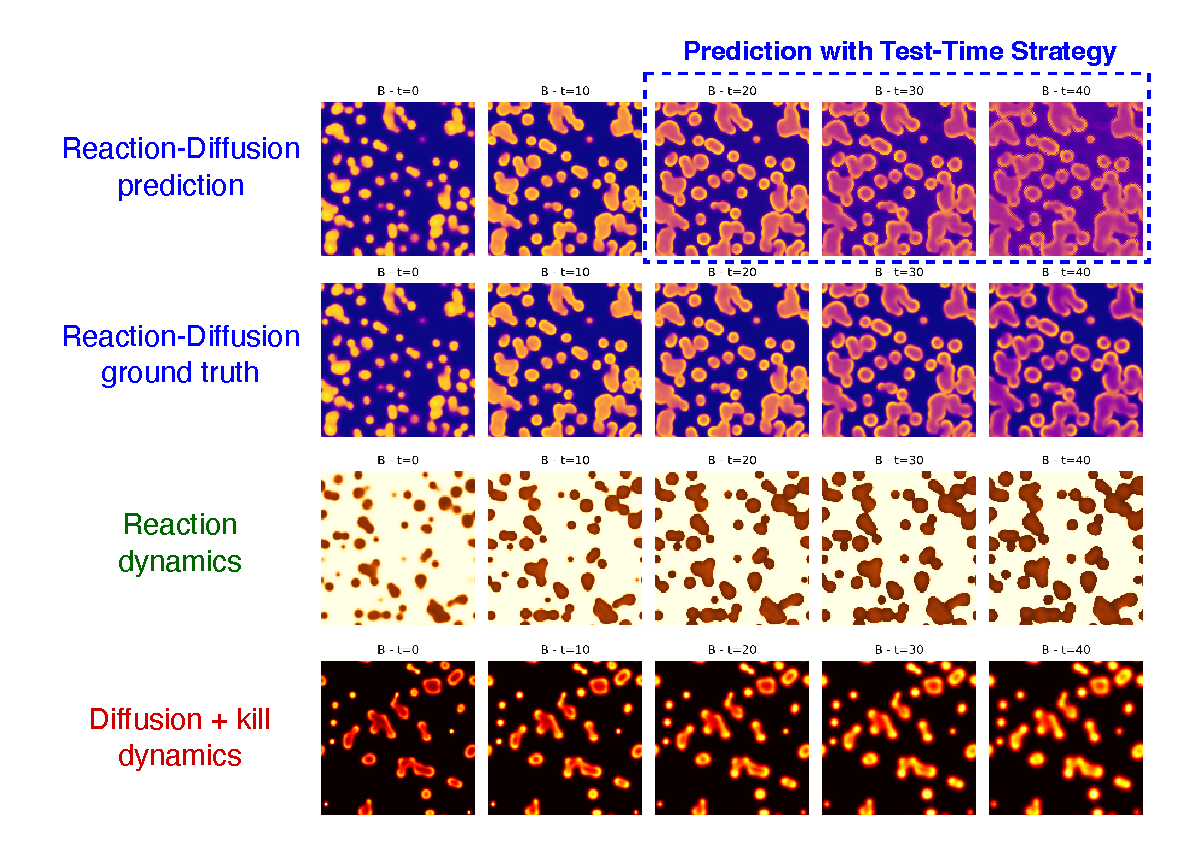
\includegraphics[width=\linewidth]{plots/zero-shot-prediction-1channel.pdf}
\caption{
%\ram{Reduce the height of the plot}
\textbf{Test-time generalization on Gray--Scott equations.}
Our neural operator search correctly predicts an unseen, non-trivial dynamics (compare first and second rows), which differs substantially from the pure reaction (third row) or pure diffusion (fourth row) seen during training, demonstrating that our method, based on combining simple operators, can capture complex phenomena.
}
\label{fig:gs-sample-trajectories}
\end{figure}

\subsection{Experimental Setting}

\label{subsec:experimental-setting}

\paragraph{Datasets.}
We design four benchmark datasets that systematically evaluate compositional generalization capabilities across different physics regimes and spatial dimensions. Each training dataset enforces strict separation of physical processes as described in \Cref{sec:problem-setting}, with operators learned exclusively from trajectories containing individual physics components, never their combinations.

\textbf{1D Advection-Diffusion.} Our first benchmark focuses on linear transport phenomena governed by $\frac{\partial u}{\partial t} = D \frac{\partial^2 u}{\partial x^2} - c \frac{\partial u}{\partial x}$ on a periodic domain of length $l=16$ with 256 spatial discretization points. Training data consists exclusively of single-physics trajectories: pure advection with speeds $c \in [0.01, 1.0]$ and zero diffusion ($D = 0$), or pure diffusion with coefficients $D \in [0.001, 1.0]$ and zero advection ($c = 0$). Each trajectory contains 100 temporal snapshots spanning $T = 10$ seconds.

\textbf{1D Combined Equation.} The second dataset examines the nonlinear advection-diffusion-dispersion equation: $\frac{\partial u}{\partial t} + \alpha \frac{\partial u^2}{\partial x} - \beta \frac{\partial^2 u}{\partial x^2} + \gamma \frac{\partial^3 u}{\partial x^3} = 0$, where $\alpha$, $\beta$, and $\gamma$ quantify the strength of nonlinear advection, diffusion, and dispersion effects, respectively. Training isolates each physical mechanism with parameter combinations $(\alpha, 0, 0)$, $(0, \beta, 0)$, and $(0, 0, \gamma)$, where coefficients are sampled uniformly from $\alpha \in [0, 1]$, $\beta \in [0, 0.4]$, and $\gamma \in [0, 1]$. We generate 8,192 training trajectories for each physics across 128 parameter configurations, with each trajectory containing 250 temporal snapshots on a 256-point spatial grid over $T=4$ seconds and a periodic domain of length $l=16$. We employ the solver from \citep{Brandstetter2022} to generate the trajectories.

\begin{figure*}
\centering
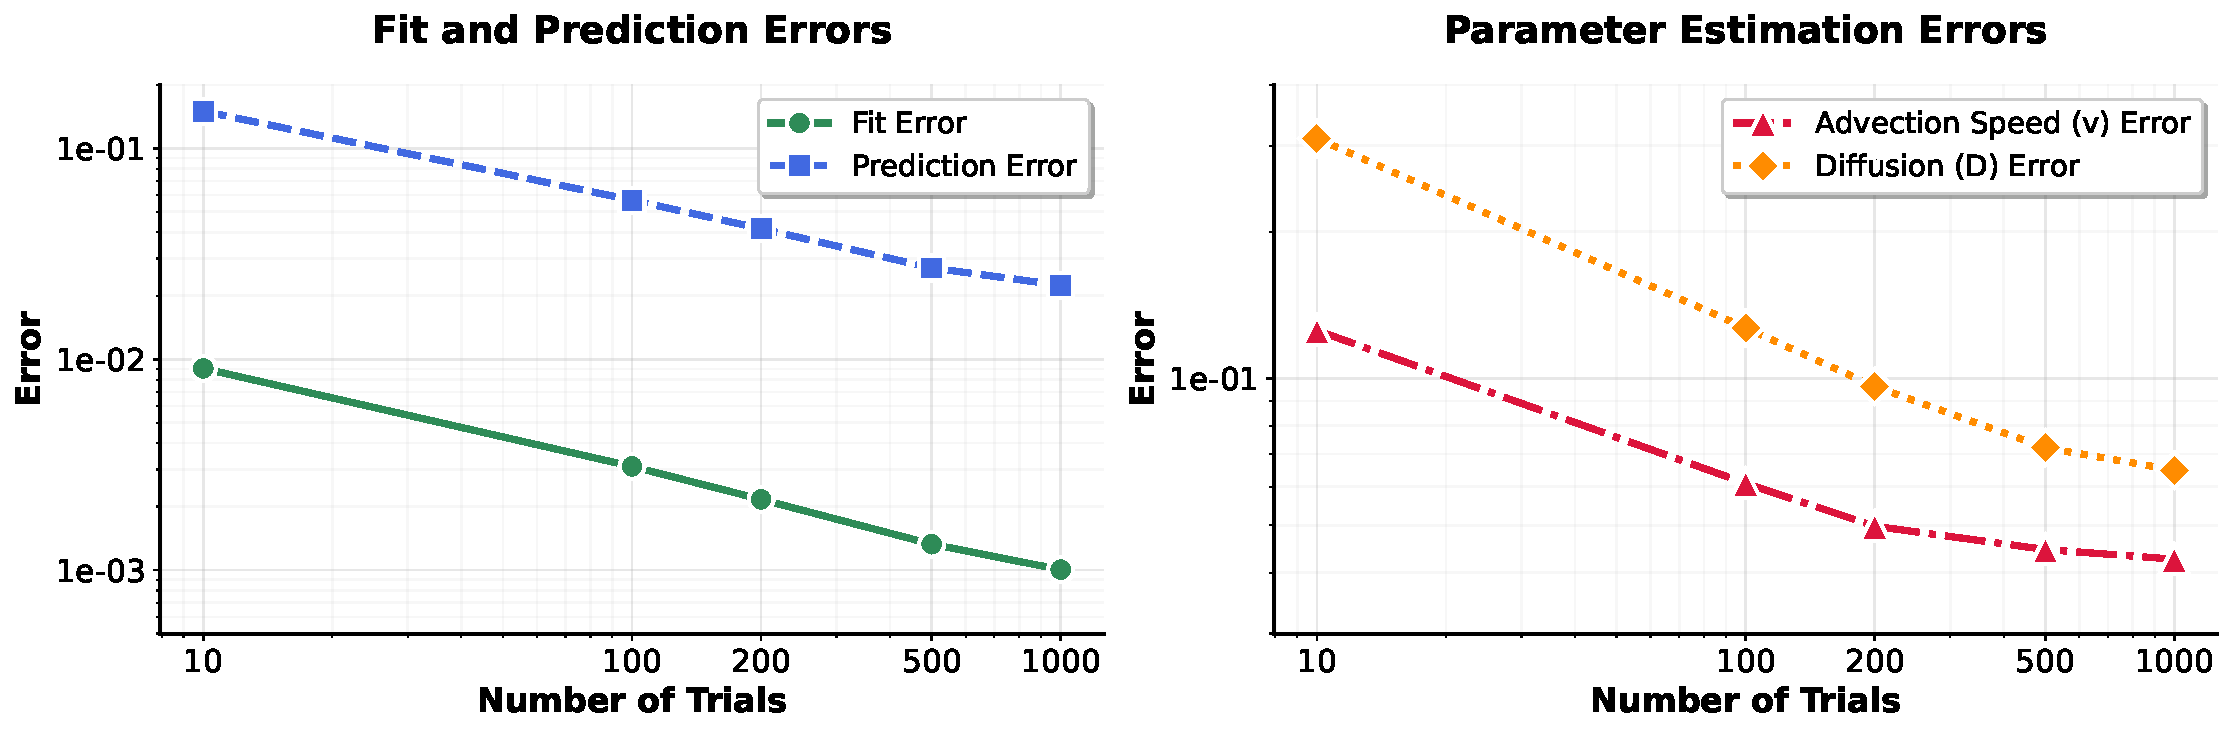
\includegraphics[width=\textwidth]{plots/error_evolution_subplots2.pdf}
\caption{
\textbf{Test-time scaling laws.} (Left) Performance of our test-time method with uniform search on an out-of-distribution (OOD) advection–diffusion dynamics. We report fitting and prediction error, measured as the mean NRMSE over 34 rollout steps, as a function of the number of uniform-search trials. (Right) Mean absolute error (MAE) for PDE parameter identification versus the number of trials, showing that the selected operators recover meaningful and accurate physical parameters. %\jh{Should the legend on right be $c$ instead of $v$?} Thank you, I will fix it when I have time.
}
\label{fig:test-time-scaling-laws}
\end{figure*}

\textbf{2D Reaction-Diffusion.} The third benchmark is the Gray--Scott reaction-diffusion equation from The Well~\citep{ohana2024well}: 
\begin{align*} 
\frac{\partial A}{\partial t} &= D_A \nabla^2 A - \delta AB^2 + F(1-A)~, \\
\frac{\partial B}{\partial t} &= D_B \nabla^2 B + \delta AB^2 - (F+k)B ~.
\end{align*} 
This system models the spatiotemporal evolution of two chemical species parameterized by diffusion coefficients $D_A, D_B$, reaction strength $\delta$, feed rate $F$ for species $A$, and kill rate $k$ for species $B$. We construct training data using two operator types: (1) diffusion-kill operators with fixed diffusion coefficients $D_A=2 \times 10^{-5}$, $D_B=1 \times 10^{-5}$, disabled reaction ($\delta = 0$, $F=0$), and kill rates $k$ spanning 20 values 
in $\{0.051, 0.052, 0.053, \ldots, 0.069, 0.070\}$; (2) pure reaction operators with disabled diffusion ($D_A=D_B=0$), unit reaction strength ($\delta = 1$), zero kill rate ($k=0$), and feed rates $F$ taking 20 values in 
$\{5, 10, \ldots, 95, 100\} \times 10^{-3}$. 
The spatial domain employs a $128 \times 128$ grid with periodic boundary conditions. We generate 512 trajectories per parameter configuration, using clustered gaussians as initial conditions, simulating for $T=50$ and keeping 50 snapshots. 

\paragraph{2D Navier--Stokes.}
Our most challenging benchmark considers a two-dimensional fluid dynamics benchmark based on the evolution of the vorticity field \(\omega(t,x,y)\) on a periodic square domain \([0,2\pi)^2\), governed by the incompressible Navier--Stokes equations in
vorticity form:
\begin{align*}
\partial_t \omega + \mathbf{u}\cdot\nabla \omega &= \nu \Delta \omega, \\
\mathbf{u} = (-\partial_y \psi,\partial_x \psi), 
\quad -\Delta \psi &= \omega .
\end{align*}
This formulation combines conservative advection and viscous diffusion.
We construct training data using two operator types: (1) \emph{pure advection} operators corresponding to the inviscid Euler equations (\(\nu=0\)), and (2) \emph{pure diffusion} operators governed by the heat equation
\(\partial_t \omega = \nu \Delta \omega\). 

Trajectories are simulated on a \(512\times512\) grid over a time horizon
\(T=4.0\), and we keep 50 snapshots, spectrally downsampled to \(256\times256\) for learning. Diffusion viscosities are sampled at 16 logarithmically spaced values in
\([10^{-4},\,10^{-2}]\), with the dataset balanced across viscosities.




% to add if Rusty comes back \newnew{\textbf{2D Navier--Stokes via Euler-Diffusion Composition.} To evaluate our method on more complex fluid dynamics, we consider the 2D incompressible Navier--Stokes equations, which can be decomposed into inviscid Euler dynamics and viscous diffusion. We train two separate neural operators: (1) a 2D Euler operator modeling inviscid flow, and (2) a 2D diffusion operator with varying diffusion coefficients. The training uses a $128 \times 128$ spatial grid with periodic boundary conditions. At test time, we compose these operators using our splitting framework to approximate Navier--Stokes dynamics across different Reynolds numbers, without any joint training or fine-tuning on the full Navier--Stokes system. We track performance across different pretraining epochs (10, 30, 50, 80, 100) to analyze how individual operator quality affects the composed system.}

\paragraph{Implementation.} 
We use the following hyperparameters for our test-time search strategies. \textbf{Uniform:} $T=100$ combinations for advection-diffusion, combined equation, and Navier--Stokes, $T=200$ for Gray--Scott, with maximum composition length $M=4$. \textbf{Beam:} We subsample $N$ operators per benchmark: 256 for advection–diffusion, 96 for the combined equation, 40 for Gray–Scott, and 17 for Navier–Stokes. We use beam width $B=4$ for advection-diffusion, combined equation, Navier--Stokes, $B=8$ for Gray--Scott, maximum composition length $M=5$, and improvement threshold of 5\%.

\paragraph{Baselines.}
We compare against different state-of-the-art approaches. All methods are trained from scratch on the same training datasets designed for this study. We use next-step prediction as the learning objective. \textbf{DISCO (Original)} \citep{morel2025disco}: We validate that our framework systematically improves upon the original DISCO approach, which performs predictions by directly encoding out-of-distribution trajectories and predicting dynamics without test-time adaptation. \textbf{MPP} \citep{mccabe2023multiple}: We compare against the Axial Vision Transformer \citep{ho2019axial} architecture designed for multiple physics pretraining, representing state-of-the-art performance in large-scale physics foundation models. \textbf{Zebra} \citep{serrano2025zebra}: We include this autoregressive transformer inspired by language modeling. While primarily designed for one-shot and few-shot adaptation for in-context learning, Zebra provides a valuable comparison as a generative model that requires higher computational resources than deterministic models. \textbf{GEPS} \citep{koupai2024geps}: We also compare against this meta-learning framework designed for efficient few-shot adaptation to changing dynamics. GEPS is trained using an environment-based perspective \citep{yin2022leads, kirchmeyer2022generalizing}, and employs a LoRA-based adaptation scheme \citep{hu2021lora}, making it a suitable comparison point for parameter efficient fine-tuning approaches.

\paragraph{Test evaluation.}
We evaluate all methods by unrolling predictions for $H$ steps per benchmark: 34 for advection–diffusion, 50 for the combined equation, 32 for Gray--Scott, and 16 for Navier--Stokes. All experiments use a history of $L=16$ snapshots as context, either for direct prediction (MPP, Zebra, original DISCO) or for adaptation (GEPS and our framework). We report the average NRMSE over the entire predicted trajectory as the primary evaluation metric.


\begin{figure}[t]
    \centering
    \begin{subfigure}{0.4\textwidth}
        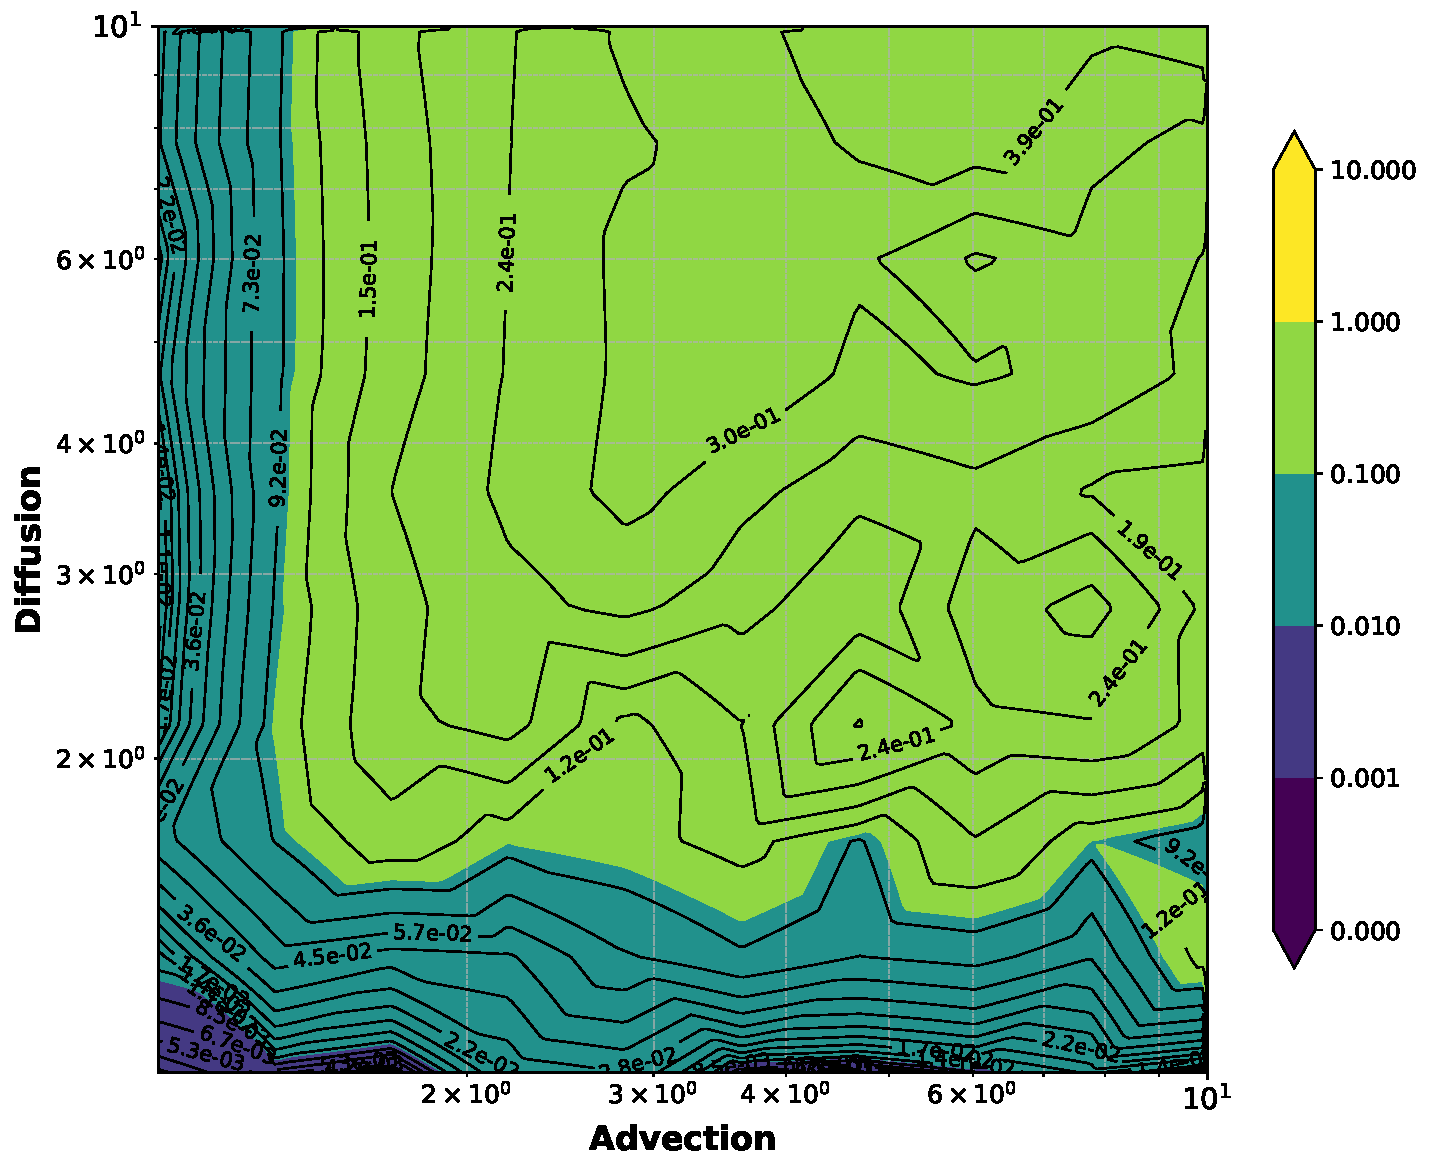
\includegraphics[width=\textwidth]{plots/direct2.pdf}
        \caption{DISCO (original) }
        \label{fig:method_a}
    \end{subfigure}
    \vfill
    \begin{subfigure}{0.4\textwidth}
        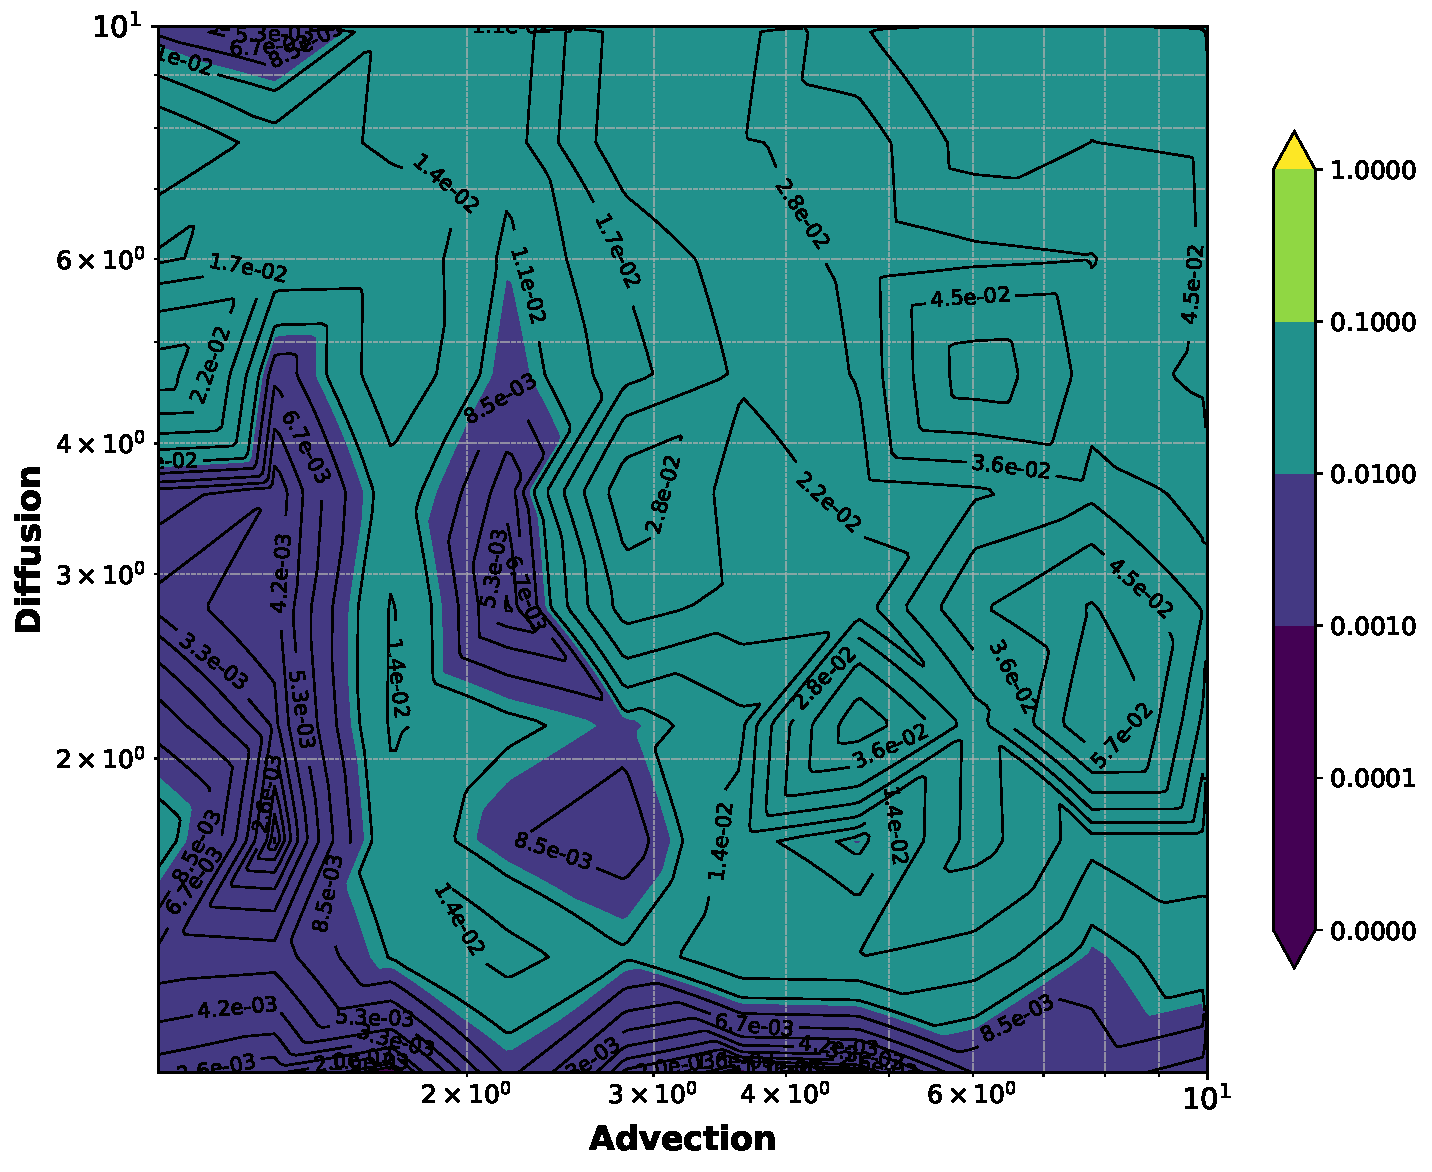
\includegraphics[width=\textwidth]{plots/beam2.pdf}
        \caption{Beam search}
        \label{fig:method_b}
    \end{subfigure}
    \caption{
\textbf{Zero-shot generalization to unseen advection-diffusion PDEs.}
Contour maps report the NRMSE (averaged over 34 rollout steps; lower is better) over the grid of advection (x-axis) and diffusion coefficients (y-axis).
(a) DISCO predictions obtained with the operator produced by the encoder and hypernetwork.
(b) Our test-time method: beam search selects operators from the dictionary to minimize the fitting error; the selected operators are then composed and unrolled via neural operator splitting.
}
\label{fig:generalization-visualization}
\end{figure}


\subsection{Parameter Extrapolation}
\label{subsec:parameter-extrapolation}

\paragraph{Setting.}
In this section, we investigate extrapolation capabilities on advection-diffusion systems by testing higher advection speeds $c \in [1, 3]$ and higher diffusion coefficients $D \in [1,3]$. While higher advection speeds present significant challenges for classical numerical solvers due to transport dominance, higher diffusion coefficients generally provide better numerical stability through smoothing effects. We also examine extrapolation performance for the nonlinear advection term $\alpha \in [1,2]$ and dispersion coefficient $\gamma \in [1,2]$ in the combined equation.

\paragraph{Results.}
Table \ref{tab:parameter_extrapolation} shows that
our test-time operator composition strategy consistently improves upon the original DISCO by orders of magnitude across all benchmarks,
demonstrating the generalization capabilities of neural operator splitting compared to direct out-of-distribution encoding. 
The beam search variant achieves the strongest performance, with improvements ranging from 11× on advection speed extrapolation to over 200× on diffusion coefficient tasks. Among the baselines, GEPS shows competitive performance on nonlinear advection and reasonable results on diffusion tasks, but exhibits instability on dispersion extrapolation. We observed that GEPS fine-tuning often leads to diverging operators during rollout for these OOD settings, consistent with previous findings on gradient-based adaptation methods \citep{serrano2025zebra}. Zebra particularly struggles on advection-diffusion tasks, which we attribute to limitations in discrete tokenization for capturing the high-frequency dynamics present in our fractal-based initial conditions. MPP provides robust but modest performance across tasks, never excelling in these extrapolation scenarios. 


\begin{table}[t]
\centering
\caption{
\textbf{Zero-shot performance on PDE parameter extrapolation.}
Average NRMSE over $H$ predicted steps (lower is better).
}
\label{tab:parameter_extrapolation}

\setlength{\tabcolsep}{5pt} % default is 6pt
\small % or \footnotesize

\begin{tabular}{lcccc}
\toprule
& \multicolumn{2}{c}{\textbf{Adv.–Diff.}} & \multicolumn{2}{c}{\textbf{Combined}} \\
\cmidrule(lr){2-3} \cmidrule(lr){4-5}
\textbf{Method} & $c$ & $D$ & $\alpha$ & $\gamma$ \\
\midrule
MPP & 0.588 & 0.409 & 0.134 & 0.369 \\
Zebra & 1.070 & 1.579 & 0.128 & 0.448 \\
GEPS & 0.848 & 0.267 & 0.020 & 0.782 \\
DISCO & 0.768 & 0.159 & 0.088 & 1.007 \\
\midrule
Ours (Uniform) & 0.113 & 0.055 & 0.027 & 0.070 \\
Ours (Beam) & \textbf{0.052} & \textbf{0.002} & \textbf{0.016} & \textbf{0.022} \\
\bottomrule
\end{tabular}
\end{table}


\subsection{Physics Composition}
\label{subsec:physics-composition}


\paragraph{Setting.}
We then evaluate the compositional capabilities of neural operators by testing their ability to combine previously isolated physical processes. For the advection-diffusion system, the test cases combine both mechanisms with coefficients sampled uniformly from $c \in [0,1]$ and $D \in [0,1]$.

For the combined equation dataset, we test four types of multi-physics compositions: (1) nonlinear advection + diffusion with $\alpha \in [0,1], \beta \in [0, 0.4]$; (2) nonlinear advection + dispersion with $\alpha \in [0,1], \gamma \in [0,1]$; (3) diffusion + dispersion with $\beta \in [0, 0.4], \gamma \in [0,1]$; and (4) all three processes combined with $\alpha \in [0,1], \beta \in [0, 0.4], \gamma \in [0,1]$. 


For the Gray–Scott system, we assess compositional generalization using test trajectories spanning the full parameter space induced by the Cartesian product of feed rates ($F$) and kill rates ($k$) from the training distribution, recombining reaction and diffusion dynamics that were seen separately.

Finally, we evaluate whether models pretrained on Euler and Diffusion 
can generalize to their composition in the 2D Navier--Stokes equations, using
matched viscosity values.


\paragraph{Results.}
Table \ref{tab:composition_results} shows that our method achieves the best performance on 5 out of 6 unseen composition tasks, with consistent improvements over the original DISCO approach. These gains are most pronounced for more complex compositions involving nonlinear or higher-order interacting terms, where directly encoding out-of-distribution trajectories often produces inaccurate or unstable operators. %In contrast, operator splitting enables explicit recombination of learned single-physics operators, yielding more reliable predictions. 
The beam search variant consistently outperforms uniform sampling, indicating that efficiently identifying a small set of compatible operators is more effective than evaluating many unstructured combinations.

Among baselines, we observe clear structural trends. MPP provides robust performance across tasks, likely due to the stability of its vision-based encoder, but lacks the compositional flexibility required to accurately model coupled dynamics. Zebra performs well on most compositions, particularly those involving nonlinear advection, reflecting the flexibility of its autoregressive formulation, though its performance degrades on more complex regimes. GEPS achieves competitive results on simpler compositions but becomes unstable as compositional complexity increases, consistent with the sensitivity of gradient-based test-time adaptation under distribution shift.

Figures~\ref{fig:gs-sample-trajectories}–\ref{fig:ns-beam-1e-3} complement the numerical results with qualitative rollouts, showing that our method qualitatively captures coupled dynamics in Gray--Scott and Navier--Stokes. Figure~\ref{fig:generalization-visualization} further demonstrates consistent improvements of the beam search over DISCO for advection--diffusion across the full coefficient range.

\subsection{Compute Scaling Analysis}
\label{subsection-scaling-analysis}


\paragraph{Test-time scaling laws.}
Figure~\ref{fig:test-time-scaling-laws} shows that increasing the number of uniform-search trials consistently reduces both fitting and prediction error, exhibiting a power-law-like decay. Moreover, improved fitting error strongly correlates with better rollout accuracy. To highlight the computational advantage of beam search over uniform search, \Cref{fig:beam-vs-uniform-scaling} plots fitting error as a function of cumulative compute (total FLOPs). Beam search rapidly outperforms uniform search by progressively expanding the operator set—first searching over single operators, then pairs, then triples, and so on—which produces sharp drops in error as more expressive combinations become available. In contrast, uniform search improves smoothly but more slowly, indicating lower compute efficiency.


\paragraph{Parameter identification.}
Beyond predictive accuracy, our method supports interpretable test-time parameter identification by tracing each selected operator to the training trajectory from which it was produced, and using that trajectory’s known physical coefficients. We estimate the coefficients of a new test trajectory by summing the parameter contributions associated with the selected operators. As shown in the right panel of Figure~\ref{fig:test-time-scaling-laws}, estimation accuracy improves as the search progresses for both the advection speed and diffusion coefficient in the advection–diffusion setting. Notably, despite never being trained on the coupled system, our method is able to recover accurate parameters for PDEs that combine these distinct physical effects.



\begin{figure}[t]
\centering
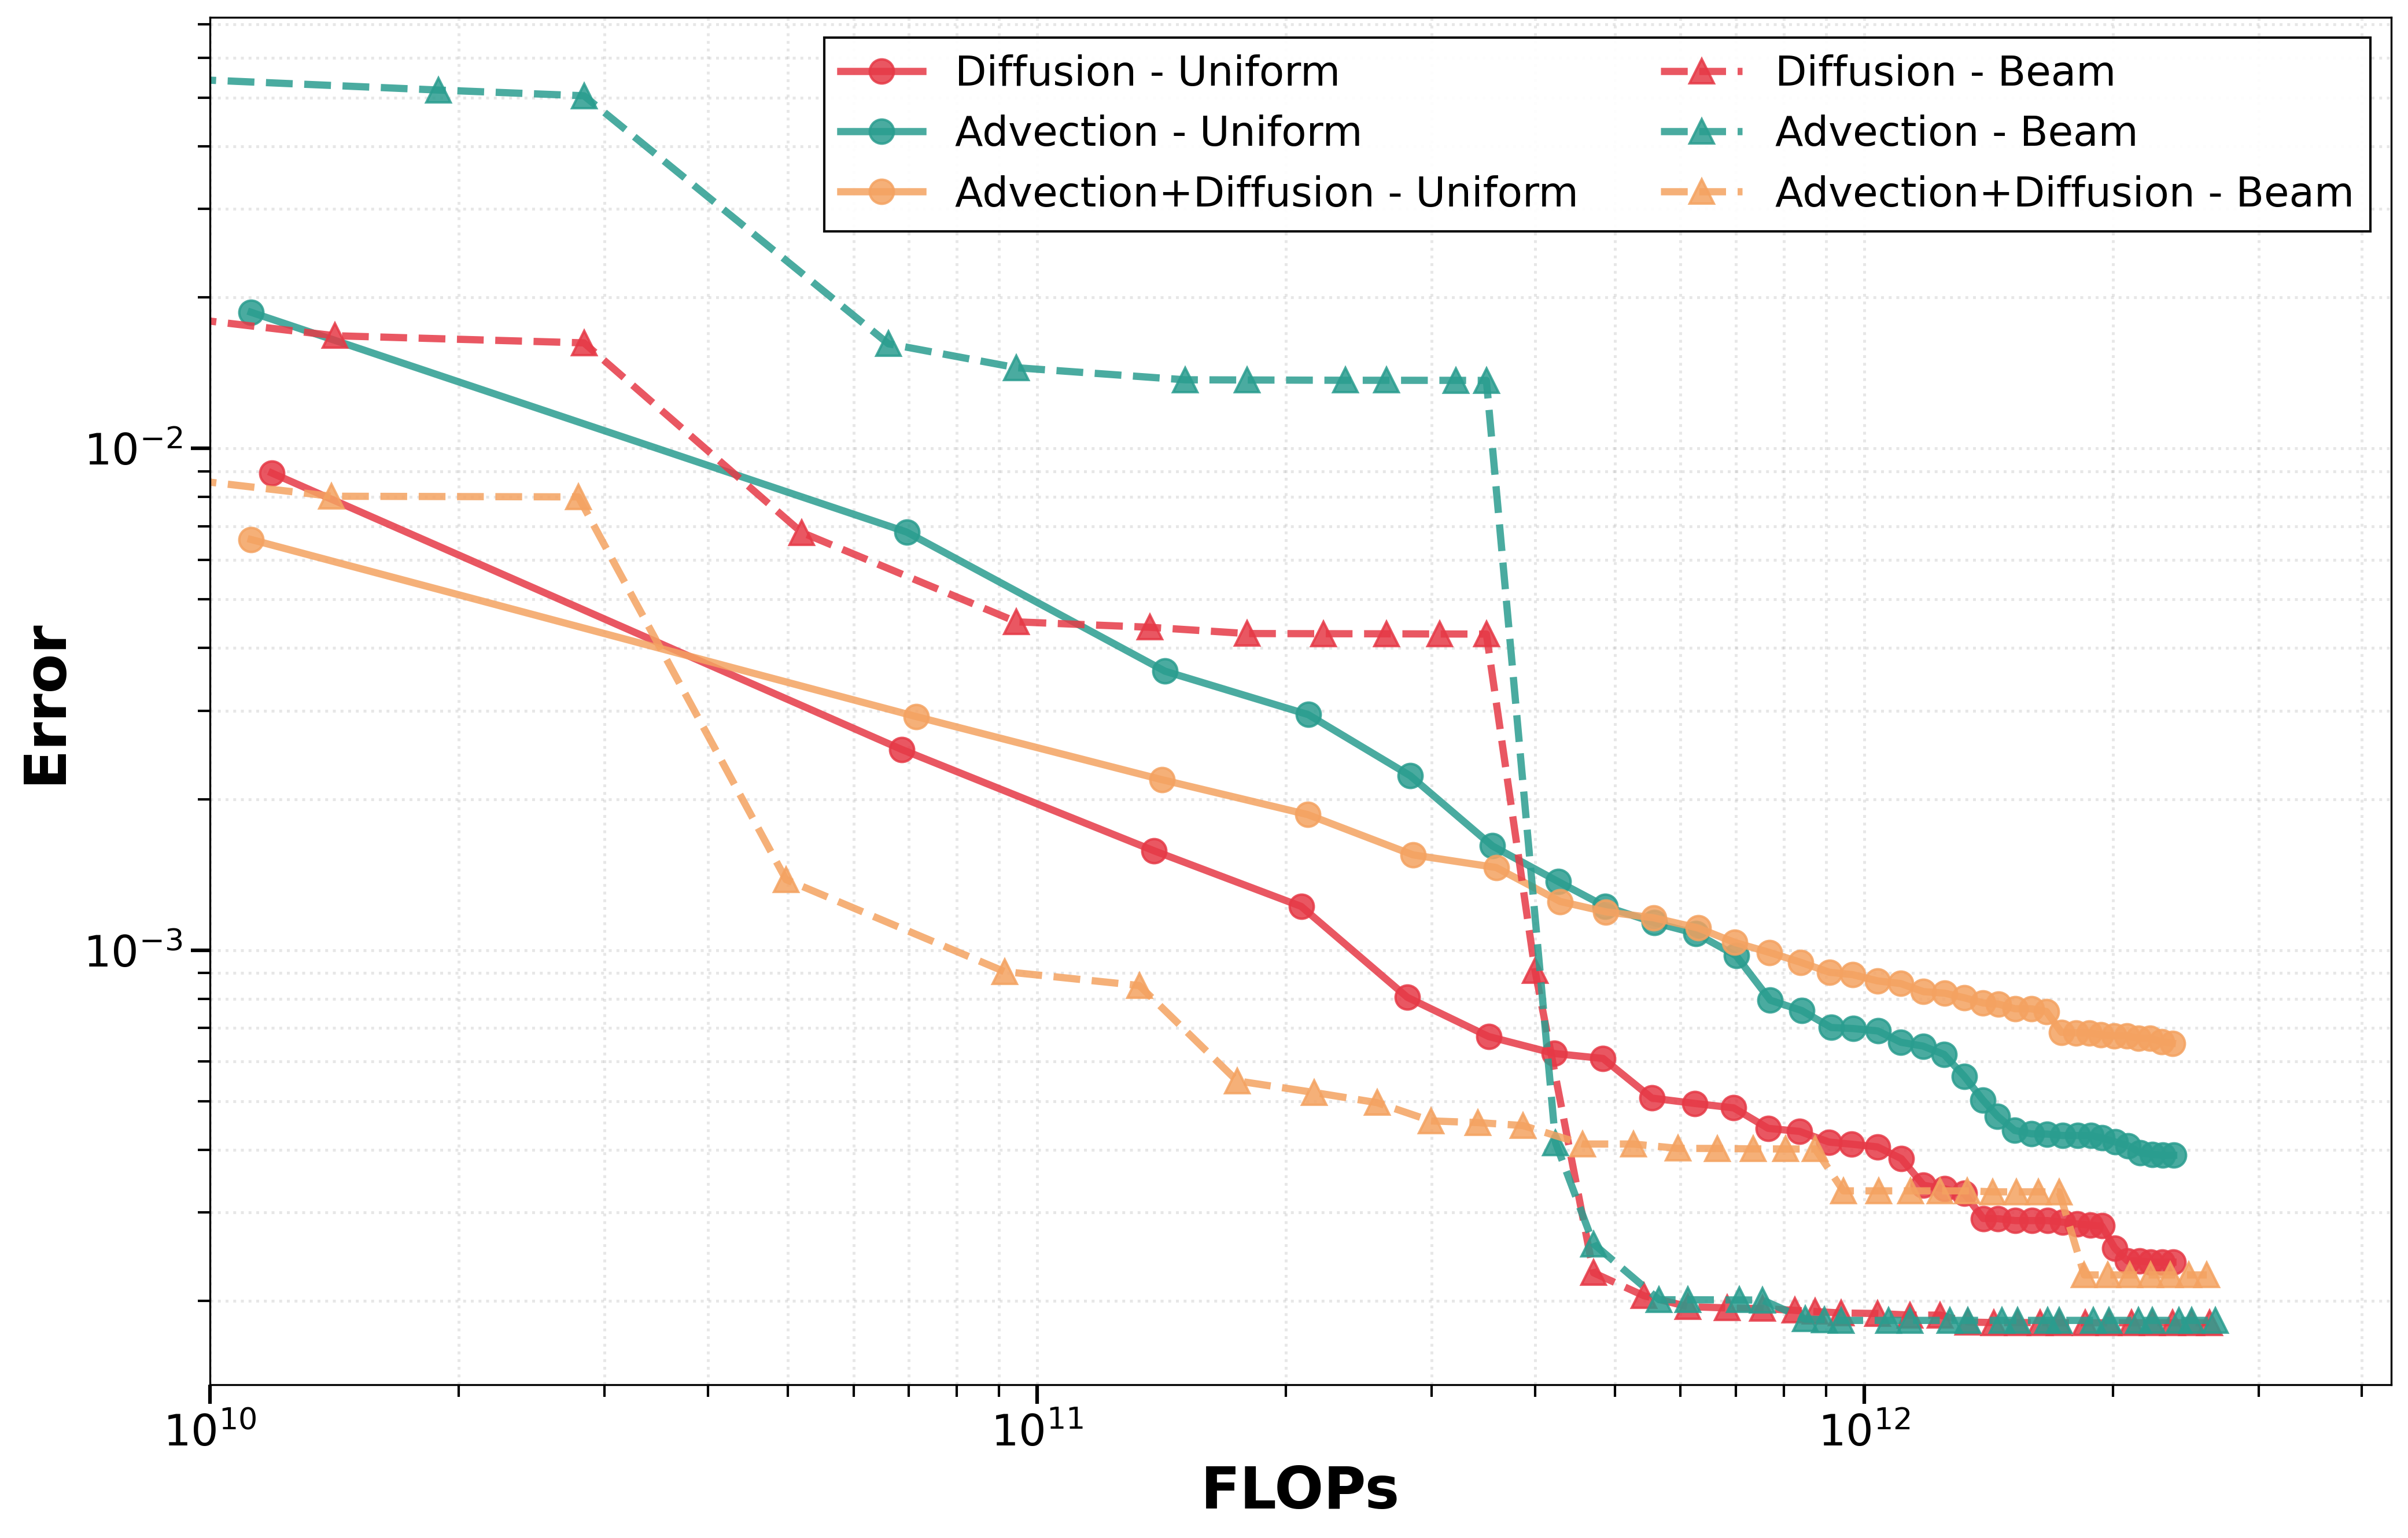
\includegraphics[width=\linewidth]{plots/flop_analysis_combined_alt-2.png}
\caption{
\textbf{Fitting error versus computational cost (FLOPs)} for uniform and beam search strategies across three tasks: diffusion extrapolation, advection extrapolation, and combined advection–diffusion. Beam search proceeds sequentially over operator complexity, first selecting the best single operators, and subsequently higher-order compositions. At intermediate FLOP budgets, beam search achieves substantially lower error than uniform search, while uniform search exhibits a smooth, approximately power-law decay with increasing computation.
}
\label{fig:beam-vs-uniform-scaling}
\end{figure}

\section{Conclusion}

We introduced a method for generalizing to out-of-distribution dynamical systems at test time without modifying model weights. 
Given a dictionary of neural operators identified at training time by a pretrained DISCO model~\cite{morel2025disco}, our method searches for combinations of these operators that best explain out-of-distribution trajectories, enabling zero-shot generalization.
Complementary to fine-tuning strategies, our method offers an additional direction for test-time generalization relying on neural operator composition and neural operator splitting.
We showed empirically that this approach achieves state-of-the-art performance on zero-shot out-of-distribution dynamics including the Navier--Stokes equations.
A current limitation is the requirement that composed operators share compatible input and output domains. 
Extending neural operator splitting to broader forms of compositionality across spatial dimensionality, discretizations, and physical fields represents a promising direction for future work.

\section*{Impact Statement}

This paper presents work whose goal is to advance the field of Machine
Learning. There are many potential societal consequences of our work, none
which we feel must be specifically highlighted here.

% In the unusual situation where you want a paper to appear in the
% references without citing it in the main text, use \nocite

\bibliography{icml2026_conference}
\bibliographystyle{icml2026}

%%%%%%%%%%%%%%%%%%%%%%%%%%%%%%%%%%%%%%%%%%%%%%%%%%%%%%%%%%%%%%%%%%%%%%%%%%%%%%%
%%%%%%%%%%%%%%%%%%%%%%%%%%%%%%%%%%%%%%%%%%%%%%%%%%%%%%%%%%%%%%%%%%%%%%%%%%%%%%%
% APPENDIX
%%%%%%%%%%%%%%%%%%%%%%%%%%%%%%%%%%%%%%%%%%%%%%%%%%%%%%%%%%%%%%%%%%%%%%%%%%%%%%%
%%%%%%%%%%%%%%%%%%%%%%%%%%%%%%%%%%%%%%%%%%%%%%%%%%%%%%%%%%%%%%%%%%%%%%%%%%%%%%%
\newpage
\appendix
\onecolumn

\section{Dataset Details}

\subsection{Advection-diffusion}

We generate synthetic trajectories for the 1D advection-diffusion equation
\begin{equation}
\frac{\partial u}{\partial t} + v \frac{\partial u}{\partial x} = D \frac{\partial^2 u}{\partial x^2}
\end{equation}
with periodic boundary conditions, where $v$ is the advection speed and $D$ is the diffusion coefficient. The dataset uses analytical solutions computed via Fourier spectral methods to avoid numerical errors.

\textbf{Physical Parameters.} During training, we generate 50\% pure advection cases ($v \sim \text{Uniform}(0.01, 1.0)$, $D = 0$) and 50\% pure diffusion cases ($v = 0$, $D \sim \text{Uniform}(0.001, 1.0)$). 

\textbf{Initial Conditions.} We generate complex initial conditions using Fractaloid with random phase patterns, which create self-similar signals with power-law spectra. These patterns are constructed as trigonometric polynomials 
\begin{equation}
u_0(x) = \sum_{k=1}^{\text{degree}} a_k k^{-\text{power}} \sin(k\theta + \phi_k),
\end{equation}
where $a_k$ are independent Gaussian coefficients and $\phi_k$ are random phases. We use $\text{degree} = 256$ and $\text{power}$ is sampled uniformly in $[1,4]$, then normalize each initial condition to zero mean and unit variance. For testing, we fix the power to $3$.

\textbf{Analytical Solutions.} We compute exact solutions using Fourier spectral methods. In spectral space, the solution evolves as $\hat{u}(k,t) = \hat{u}_0(k) \exp(-Dk^2t) \exp(-ikvt)$, which we transform back to physical space via inverse FFT. The spatial domain has length $L = 16.0$ with $n_x = 256$ grid points, evolved over $n_t = 100$ time steps to final time $T = 10.0$.


\subsection{Combined-equation}

We follow the dataset generation approach of \cite{Brandstetter2022}, with key distinctions in the physics formulation for training data generation and the exclusion of forcing terms. The combined equation is governed by the following PDE:
\begin{equation}
\partial_t u + \partial_x (\alpha u^2 - \beta \partial_x u + \gamma \partial_{xx} u) = 0,
\end{equation}
subject to periodic boundary conditions and initial conditions
\begin{equation}
\label{equation:init}
u_0(x) = \sum_{j=1}^{J} A_j \sin(2\pi \ell_j x / l + \phi_j).
\end{equation}

This formulation combines three fundamental physical mechanisms: nonlinear advection ($\alpha u^2$), linear diffusion ($-\beta \partial_x u$), and dispersion ($\gamma \partial_{xx} u$). For each initial condition, we sample the Fourier mode coefficients: $A_j \sim \text{Uniform}([-0.5, 0.5])$, $\ell_j \sim \text{Uniform}(\{1, 2, 3, 4, 5\})$, and $\phi_j \sim \text{Uniform}([0, 2\pi])$ with $J=5$ modes.

\textbf{Training dataset} The training data is generated using parameter combinations $(\alpha, 0, 0)$, $(0, \beta, 0)$, and $(0, 0, \gamma)$. The coefficients are sampled uniformly from $\alpha \in [0, 1]$, $\beta \in [0, 0.4]$, and $\gamma \in [0, 1]$. We generate 8,192 training trajectories for each isolated physics across 128 parameter configurations. Each trajectory contains 250 temporal snapshots on a 256-point spatial grid over $T=4$ seconds with a periodic domain of length $l=16$.

\subsection{Reaction-Diffusion}

Our most challenging benchmark is the Gray--Scott reaction-diffusion system from The Well~\citep{ohana2024well}: 
\begin{align} 
\frac{\partial A}{\partial t} &= D_A \nabla^2 A - \delta AB^2 + F(1-A), \\
\frac{\partial B}{\partial t} &= D_B \nabla^2 B + \delta AB^2 - (F+k)B.
\end{align} 
This system models the spatiotemporal evolution of two chemical species parameterized by diffusion coefficients $D_A, D_B$, reaction strength $\delta$, feed rate $F$ for species $A$, and kill rate $k$ for species $B$. 

\textbf{Training Data Generation.} We construct training data using two types of operators. First, \textit{diffusion-kill operators} use fixed diffusion coefficients $D_A=2 \times 10^{-5}$, $D_B=1 \times 10^{-5}$, disabled reaction terms ($\delta = 0$, $F=0$), and kill rates $k$ spanning 20 values in $\{0.051, 0.052, \ldots, 0.070\}$. Second, \textit{pure reaction operators} disable diffusion ($D_A=D_B=0$), set unit reaction strength ($\delta = 1$), zero kill rate ($k=0$), and vary feed rates $F$ across 20 values in $\{5, 10, \ldots, 100\} \times 10^{-3}$.

The spatial domain employs a $128 \times 128$ grid with periodic boundary conditions. We generate 512 trajectories per parameter configuration, simulating 50 seconds and retaining 50 temporal snapshots using the solver from \citet{ohana2024well}.

\textbf{Initial Conditions.} To ensure fair evaluation of dynamics identification and extrapolation capabilities, we address the distinct field characteristics produced by reaction versus diffusion dynamics. We begin with clustered Gaussian initial conditions, then evolve them for a random duration between 0 and 100 seconds using the full reaction-diffusion dynamics. The resulting evolved states serve as initial conditions for generating the isolated reaction and diffusion training trajectories. This procedure mitigates potential frequency bias across all methods and enables the assessment of operator learning rather than initial condition adaptation.


\subsection{Euler, Diffusion, and Navier--Stokes Equations}

All data consist of trajectories of the two-dimensional vorticity field
\(\omega(t,x,y)\) on a periodic square domain \([0,2\pi)^2\).

\paragraph{Euler equations (inviscid).}
The 2D incompressible Euler equations are solved in vorticity form:
\begin{equation}
\partial_t \omega + \mathbf{u}\cdot\nabla \omega = 0,
\qquad
\mathbf{u} = (-\partial_y \psi,\; \partial_x \psi),
\qquad
-\Delta \psi = \omega .
\end{equation}

\paragraph{Diffusion equation.}
For the purely dissipative components, we also generate trajectories of the heat
equation
\begin{equation}
\partial_t \omega = \nu \Delta \omega ,
\end{equation}
where \(\nu > 0\) denotes the diffusion coefficient.

\paragraph{Navier--Stokes equations.}
We consider the two-dimensional incompressible Navier--Stokes equations as the
viscous extension of the Euler equations, also written in vorticity form:
\begin{equation}
\partial_t \omega + \mathbf{u}\cdot\nabla \omega = \nu \Delta \omega ,
\qquad
\mathbf{u} = (-\partial_y \psi,\; \partial_x \psi),
\qquad
-\Delta \psi = \omega .
\end{equation}

\paragraph{Numerical Discretization.}
All simulations are performed using a Fourier pseudo-spectral method on a
uniform \(512 \times 512\) grid. Spatial derivatives are computed exactly in
Fourier space, while nonlinear terms are evaluated in physical space.

For Euler and Navier--Stokes simulations, the nonlinear advection term is
dealiased using the standard \(3/2\)-rule padding. Time integration is carried
out using an implicit midpoint scheme, solved via fixed-point iterations in
spectral space. This method improves long-time stability and preserves
invariants in the inviscid limit. The timestep is chosen adaptively according to
a CFL condition, with an additional diffusion stability constraint when
\(\nu>0\).

The diffusion equation is solved exactly in Fourier space using the closed-form
solution
\begin{equation}
\hat{\omega}(t,k) = \hat{\omega}(0,k)\exp\!\left(-\nu |k|^2 t\right),
\end{equation}
which introduces no time-discretization error beyond floating-point precision.

\paragraph{Initial Conditions.}
Initial vorticity fields are smooth and periodic. Euler initial conditions are
generated as random low-frequency Fourier-mode mixtures of the form
\begin{equation}
\omega_0(x,y) =
\sum_{n,m=1}^{N_m} a_{nm}
\sin\!\left(\tfrac{2\pi n}{L}x + \phi_{nm}\right)
\sin\!\left(\tfrac{2\pi m}{L}y + \psi_{nm}\right),
\end{equation}
where amplitudes \(a_{nm}\) are Gaussian with variance proportional to
\(10\,(n+m)^{-1}\), and phases \(\phi_{nm}, \psi_{nm}\) are sampled uniformly from
\([0,2\pi)\). This construction ensures spatial smoothness and exact
periodicity. We use \(N_m = 5\) modes for all smooth initial conditions.

Diffusion initial conditions are obtained by sampling random intermediate
snapshots (uniformly in time) from Euler trajectories. This yields physically
realistic initial states containing coherent vortical structures and a broad
range of spatial scales.

\paragraph{Time Horizon and Downsampling.}
Each trajectory is evolved over a fixed time horizon \(T = 4.0\) and recorded at
\(n_{\text{snap}} = 50\) uniformly spaced time points.

For storage and learning, trajectories are downsampled to a lower output
resolution (e.g., \(256 \times 256\)) using spectral truncation. Fourier modes
outside the target bandwidth are removed, and the field is reconstructed via
inverse FFT. This procedure preserves large-scale dynamics and avoids aliasing
artifacts.

\paragraph{Diffusion Viscosities} Diffusion trajectories for both the diffusion and Navier--Stokes datasets are
generated for viscosities \(\nu\) logarithmically spaced in the interval
\([10^{-4}, 10^{-2}]\). The dataset is balanced such that an equal number of
trajectories is generated for each viscosity value.




\section{Implementation Details}

\subsection{DISCO implementation}

\paragraph{Hyperparameters} We use the recommended default configuration from \cite{morel2025disco} with targeted modifications for our experiments. For the transformer encoder, we employ a hidden dimension of 128, patch sizes of 8 in 1D and $8 \times 8$ in 2D, and 4 encoder blocks with 4 attention heads each using relative position bias. We introduce a bottleneck projection layer that reduces the 128-dimensional transformer output to $C$ channels, where $C = \{2, 3, 2\}$ for advection-diffusion, combined-equation, and reaction-diffusion respectively. This bottleneck layer is inserted before DISCO's original MLP decoder, representing a minimal architectural change that improves generalization across initial conditions.

For the neural ODE component, we select the RK4 solver with problem-specific integration time spans: $dt = \{0.1, 0.016, 1\}$ for advection-diffusion, combined-equation, and reaction-diffusion respectively. We apply periodic boundary conditions and configure the operator network with 8 base channels and a $2\times$ bottleneck multiplier for efficient ODE parameter prediction from transformer representations.

We train models for 300,000 iterations on advection-diffusion and combined-equation tasks, and 100,000 iterations for reaction-diffusion. We use AdamW optimizer with a base learning rate of $3 \times 10^{-4}$, cosine annealing scheduler, and weight decay of $1 \times 10^{-4}$.

\subsection{Training recipe}
The original DISCO training procedure uses the operator to predict the frame immediately following the input encoder sequence. We found that increasing input diversity to the operator network produces more robust operators that generalize across different initial conditions.

We therefore propose an alternative training strategy based on contextual learning. For advection-diffusion equations, we sample two trajectories that follow identical dynamics: we encode trajectory 1 with the hypernetwork to obtain an operator, then apply this operator to predict the next timestep of trajectory 2. This in-context approach draws inspiration from \citet{serrano2025zebra}.

For Combined-equation and Gray--Scott systems, we adopt an environment-based training paradigm to enable fair comparison with GEPS \cite{koupai2024geps}. We assume knowledge of which trajectories belong to the same environment and implement a codebook updated via exponential moving average following \cite{oord2017neural}. During training, we randomly select either the encoder-derived code (50\% probability) or the corresponding environment code from the codebook (50\% probability), ensuring the encoder learns meaningful representations while maintaining environment consistency.



\begin{algorithm}
\small
\caption{Beam Search Operator Composition}
\label{alg:beam_search}
\begin{algorithmic}[1]
\REQUIRE Test trajectory $u_{\text{test}}^{1:L}$, dictionary $\{f_1, \ldots, f_N\}$, beam width $B$, max iterations $M$, threshold $\tau$
\ENSURE Best operator subset $S^*$
\STATE Initialize: $\mathcal{B}_0 = \text{top-}B \text{ operators ranked by } \mathcal{L}(\{f_i\})$
\FOR{$m = 0$ to $M-1$}
    \STATE Candidates $= \emptyset$
    \FOR{each $S \in \mathcal{B}_m$}
        \FOR{each $f_j \in \{f_1, \ldots, f_N\} \setminus S$}
            \STATE Add $S \cup \{f_j\}$ to Candidates
        \ENDFOR
    \ENDFOR
    \STATE $\mathcal{B}_{m+1} = \text{top-}B \text{ from Candidates ranked by } \mathcal{L}(\cdot)$
    \IF{relative improvement $ < \tau$ or $m = M-1$}
        \STATE \textbf{break}
    \ENDIF
\ENDFOR
%\RETURN toto
\RETURN $\argmin_{S \in \mathcal{B}_m} \mathcal{L}(S)$
\end{algorithmic}
\end{algorithm}


\begin{algorithm}
\caption{Uniform Operator Composition Search}
\label{alg:random_search}
\begin{algorithmic}[1]
\REQUIRE Test trajectory $u_{\text{test}}^{1:L}$, operator dictionary $\{f_1, \ldots, f_N\}$, number of trials $N_{\text{trials}}$, maximum composition length $M$
\ENSURE Best operator subset $S^*$
\STATE Initialize best operator subset $S^* = \{\argmin_{f_i \in \{f_1, \ldots, f_N\}} \mathcal{L}(\{f_i\})\}$
\STATE Initialize best loss $\mathcal{L}^* = \mathcal{L}(S^*)$
\FOR{$i = 1$ to $N_{\text{trials}}$}
    \STATE Sample composition length $m \sim \text{Uniform}(\{1, 2, \ldots, M\})$
    \STATE Sample operator subset $S_i \sim \text{Uniform}(\text{subsets of } \{f_1, \ldots, f_N\} \text{ with size } m)$
    \STATE Compute loss $\mathcal{L}_i = \mathcal{L}(S_i)$
    \IF{$\mathcal{L}_i < \mathcal{L}^*$}
        \STATE $S^* = S_i$
        \STATE $\mathcal{L}^* = \mathcal{L}_i$
    \ENDIF
\ENDFOR
\RETURN $S^*$
\end{algorithmic}
\end{algorithm}


\subsection{Operator splitting with $m$ operators}
\label{subsection-multiple-operator splitting}

For multiple operators $f_{i_1} + f_{i_2} + \cdots + f_{i_m}$, we generalize the composition by sequentially composing the individual operator flows.
The Lie splitting for $m$ operators is given by
\[
\hat{u}^{L+1}
=
f_{i_m}^{\Delta t}
\circ
f_{i_{m-1}}^{\Delta t}
\circ \cdots \circ
f_{i_1}^{\Delta t}
\left(u^L\right),
\]
yielding a first-order approximation of the full evolution operator.

To obtain second-order accuracy, we employ a symmetric Strang-type splitting for multiple operators:
\[
\hat{u}^{L+1}
=
f_{i_1}^{\Delta t/2}
\circ
f_{i_2}^{\Delta t/2}
\circ \cdots \circ
f_{i_{m-1}}^{\Delta t/2}
\circ
f_{i_m}^{\Delta t}
\circ
f_{i_{m-1}}^{\Delta t/2}
\circ \cdots \circ
f_{i_1}^{\Delta t/2}
\left(u^L\right).
\]
This palindromic composition preserves the symmetry required for second-order accuracy and extends classical Strang splitting to multiple operators \citep{Strang1968OnTC, Marchuk1990SplittingAA}.


\subsection{Baselines}

\paragraph{MPP} We use the recommended default hyperparameters with periodic boundary conditions and 6 encoder blocks, employing a hidden dimension of 384 for 2D experiments, and train for 100,000 iterations using AdamW optimizer with a learning rate of $5 \times 10^{-4}$ and batch size of 64.

\paragraph{Zebra} We adopt the recommended default configuration, using 64, 32, and 256 tokens respectively to encode each frame for advection-diffusion, combined-equation, and reaction-diffusion tasks. We train without in-context examples, employing maximum history lengths of 50, 66, and 32 frames for advection-diffusion, combined-equation, and reaction-diffusion respectively. At inference, we sample the next token from the multinomial distribution with a temperature of 0.1 to reduce the variance.

\paragraph{GEPS} We use the CNN1D and CNN2D implementations from the original codebase, training for 100,000 steps with AdamW optimizer and cosine learning rate scheduling. Since GEPS requires environment information during training, we provide labels indicating which trajectories belong to the same environment. At inference, we address rollout instabilities by performing multiple optimization runs (100, 500, and 2000 gradient steps) and report the best test set performance across these attempts.

\section{Additional Experimental results}


% \subsection{Computational Scaling Analysis}
% \label{subsec:compute-overhead}

% A central question for test-time adaptation is how accuracy scales with additional computation. We analyze this tradeoff on the advection–diffusion composition task, focusing on qualitative differences between gradient-based adaptation and search-based test-time methods.


% \paragraph{Comparison with baselines.}
% In Table~\ref{tab:compute_overhead}, the results show three distinct operating regimes. Direct prediction operates in a low-compute regime but fails to achieve meaningful accuracy under distribution shift. GEPS fine-tuning substantially improves performance at moderate computational cost, but remains bounded in its achievable error. In contrast, our test-time search methods operate in a higher-compute regime where accuracy continues to improve as more resources are allocated. Among these, beam search consistently provides the best accuracy–compute balance, while uniform sampling incurs additional cost with diminishing returns.



% \begin{table}[t]
% \centering
% \caption{
% \textbf{Compute-accuracy comparison.}
% Final computational cost (FLOPs in billions) and prediction error (NRMSE) for different methods on advection-diffusion composition.
% }
% \label{tab:compute_overhead}
% \begin{tabular}{@{}lcc@{}}
% \toprule
% \textbf{Method} & \textbf{FLOPs (B)} & \textbf{Final Error} \\
% \midrule
% Direct (DISCO) & 0.34 & 9.99e-02 \\
% GEPS fine-tuning & 161.15 & 2.81e-03 \\
% Beam Search (Ours) & 612.60 & 4.65e-04 \\
% Random (Ours) & 951.68 & 1.22e-03 \\
% \bottomrule
% \end{tabular}
% \end{table}

% \paragraph{Scaling behavior.}
% Figure~\ref{fig:compute_scaling} highlights a key qualitative difference in scaling. GEPS exhibits early saturation: beyond a limited number of fine-tuning steps, additional computation does not translate into further error reduction. Our methods, by contrast, show smooth and monotonic improvement as the test-time budget increases. This behavior suggests that discrete operator search remains effective even when gradient-based adaptation has converged, enabling continued refinement in far out-of-distribution settings.


% % \begin{figure}[t]
% % \centering
% % \includegraphics[width=0.9\linewidth]{plots/compute_scaling_comparison.pdf}
% % \caption{
% % \textbf{Compute scaling comparison.}
% % Error vs. FLOPs for test-time methods (beam search, uniform sampling) and GEPS fine-tuning. Our methods improve monotonically with compute while GEPS plateaus early.
% % }
% % \label{fig:compute_scaling}
% % \end{figure}

% Overall, these results indicate that our approach operates in a favorable test-time compute regime, where additional resources reliably improve accuracy. This property is particularly valuable in settings where inference-time computation can be flexibly traded for precision. The observed plateau of GEPS further suggests that local optimization alone is insufficient to recover high-quality solutions under severe distribution shift, whereas explicit exploration over operator compositions remains effective.



%\subsection{Navier--Stokes Approximation via Euler-Diffusion Composition}
%\label{subsec:Navier--Stokes}

%We next evaluate whether neural operator splitting can recover more complex fluid dynamics by composing operators trained on simpler physical processes. Specifically, we test whether separately trained Euler and diffusion operators can be combined to approximate 2D incompressible Navier–Stokes dynamics.


%\paragraph{Setting.}
%The Navier–Stokes equations naturally decompose into inviscid transport and viscous diffusion. We exploit this structure by training two independent neural operators—one for 2D Euler dynamics and one for diffusion—without exposing either model to the full Navier–Stokes system. At test time, we compose these operators using Strang splitting, without any joint training or parameter updates.


%\paragraph{Results.}
%The composed solver exhibits consistent improvement as the quality of the underlying operators increases. Improvements in the Euler and diffusion components translate directly into lower error for both single-step prediction and long-horizon rollouts. Notably, the composed model achieves stable Navier–Stokes trajectories despite never being trained on the target system, indicating that additive operator composition is sufficiently expressive to capture nontrivial fluid dynamics.


%\begin{table}[t]
%\centering
%\caption{
%\textbf{Navier--Stokes approximation via neural operator splitting.}
%Performance of composed Navier--Stokes solver using separately trained Euler2D and Diffusion2D operators across different pretraining epochs. Neither operator was trained on the full Navier--Stokes system.
%}
%\label{tab:navier_stokes}
%\setlength{\tabcolsep}{5pt} % default is 6pt
%\small % or \footnotesize
% \begin{tabular}{@{}ccccc@{}}
% \toprule
% \textbf{Epoch} & \textbf{Euler2D Err} & \textbf{Diff2D Err} & \textbf{NS Next-Step} & \textbf{NS Rollout} \\
% \midrule
% 10 & 1.42e-02 & 1.38e-03 & 1.26e-02 & 3.17e-01 \\
% 30 & 8.99e-03 & 1.27e-04 & 9.08e-03 & 2.46e-01 \\
% 50 & 7.66e-03 & 4.07e-05 & 7.10e-03 & 1.84e-01 \\
% 80 & 6.86e-03 & 2.23e-05 & 6.53e-03 & 1.76e-01 \\
% 100 & 6.55e-03 & 2.10e-05 & 6.42e-03 & 1.73e-01 \\
% \bottomrule
% \end{tabular}
% \end{table}

% These results \Cref{subsec:splitting-accuracy} demonstrate that neural operator splitting can successfully transfer knowledge from isolated physical subsystems to more complex dynamics. Moreover, the smooth dependence on pretraining quality suggests that composition behaves predictably, rather than introducing instability or compounding errors.
% }

\subsection{Splitting Accuracy and Individual Operator Quality}
\label{subsec:splitting-accuracy}

We investigate how approximation error in individual learned neural operators influences the accuracy of their composition. Although operator splitting is well studied in classical numerical analysis, the extent to which splitting interacts with learned operator error is not obvious \emph{a priori} and therefore benefits from empirical evaluation.



\paragraph{Experimental setup.}
We consider a 1D heat--dispersion system and train separate neural operators for each component over multiple pretraining epochs, producing operators with varying levels of accuracy. At evaluation time, we compose these learned components using Strang splitting, and report both single-step prediction error and long-horizon rollout error (250 steps).



\paragraph{Results.}
Overall, the accuracy of the composed system largely tracks the least accurate constituent operator. In particular, when one component exhibits substantially higher error than the other, the splitting error is typically governed by that weaker operator, even when the second component is already highly accurate. As both operators improve with continued pretraining, the composed error decreases consistently and proportionally. We note one exception at the highest-accuracy setting (last row of \Cref{tab:splitting_accuracy}), where the composed error is slightly lower than the larger of the two individual operator errors, suggesting that composition can occasionally be marginally better than a strict ``worst-operator'' bound. Nonetheless, the overall trend remains stable, with no evidence of unexpected degradation from composition.




\begin{table}[t]
\centering
\caption{
\textbf{Operator splitting accuracy vs. individual operator quality.}
Composition of heat diffusion and dispersion operators across pretraining epochs. The composed system's error is dominated by the least accurate individual operator.
}
\label{tab:splitting_accuracy}
\setlength{\tabcolsep}{5pt} % default is 6pt
\small % or \footnotesize
\begin{tabular}{@{}ccccc@{}}
\toprule
\textbf{Epoch} & \textbf{Heat Err} & \textbf{Dispersion Err} & \textbf{Split Next-Step} & \textbf{Split Rollout} \\
\midrule
50 & 5.39e-05 & 1.47e-03 & 1.24e-03 & 1.22e-01 \\
150 & 3.45e-05 & 1.02e-03 & 8.46e-04 & 1.02e-01 \\
250 & 2.08e-05 & 6.18e-04 & 6.55e-04 & 9.90e-02 \\
350 & 5.84e-06 & 1.52e-04 & 1.93e-04 & 2.73e-02 \\
500 & 2.59e-06 & 8.95e-05 & 8.26e-05 & 8.85e-03 \\
\bottomrule
\end{tabular}
\end{table}

\paragraph{Interpretation}
These results demonstrate a clear ``weakest-link'' behavior in learned operator splitting: improvements to an already accurate component yield limited overall benefit unless the less accurate operator is also improved. At the same time, the monotonic reduction in error across training stages suggests that Strang splitting does not introduce pathological interactions between learned operators. Overall, this supports the practical value of modular training, while highlighting that performance gains in composed systems are driven primarily by progress on the most challenging component.




\section{Qualitative results}

\paragraph{Combined equation} We can see in \Cref{fig:diffusion+dispersion} , \ref{fig:nonlinear+dispersion}, \ref{fig:nonlinear+diffusion+dispersion}, \ref{fig:nonlinear+diffusion} that our test-time operator splitting strategy demonstrates remarkable capability in matching ground truth dynamics over extended rollouts, despite operating out-of-distribution and being trained solely for single-step prediction. The model maintains high fidelity predictions throughout the majority of the 100-step rollout, with some error accumulation becoming visible after approximately 70 timesteps, which is expected for such long-horizon extrapolation tasks.

\paragraph{Reaction diffusion} We provide an augmented comparison of the dynamics seen during training with the second channel in \Cref{fig:zero-shot-prediction-2channels}. We also show additional comparisons of predictions and ground truths in \Cref{fig:gs-sample0}, \ref{fig:gs-sample55}, \ref{fig:gs-sample62}.


\paragraph{Navier--Stokes} Figures~\ref{fig:ns-beam-1e-2}, \ref{fig:ns-direct-1e-2}, \ref{fig:ns-beam-1e-3}, and \ref{fig:ns-direct-1e-3} contrast direct predictions with our test-time strategy for OOD Navier–Stokes trajectories. The test-time strategy achieves lower error, and the qualitative improvement is especially noticeable in the higher-viscosity regime.

\begin{figure}[h]
\centering
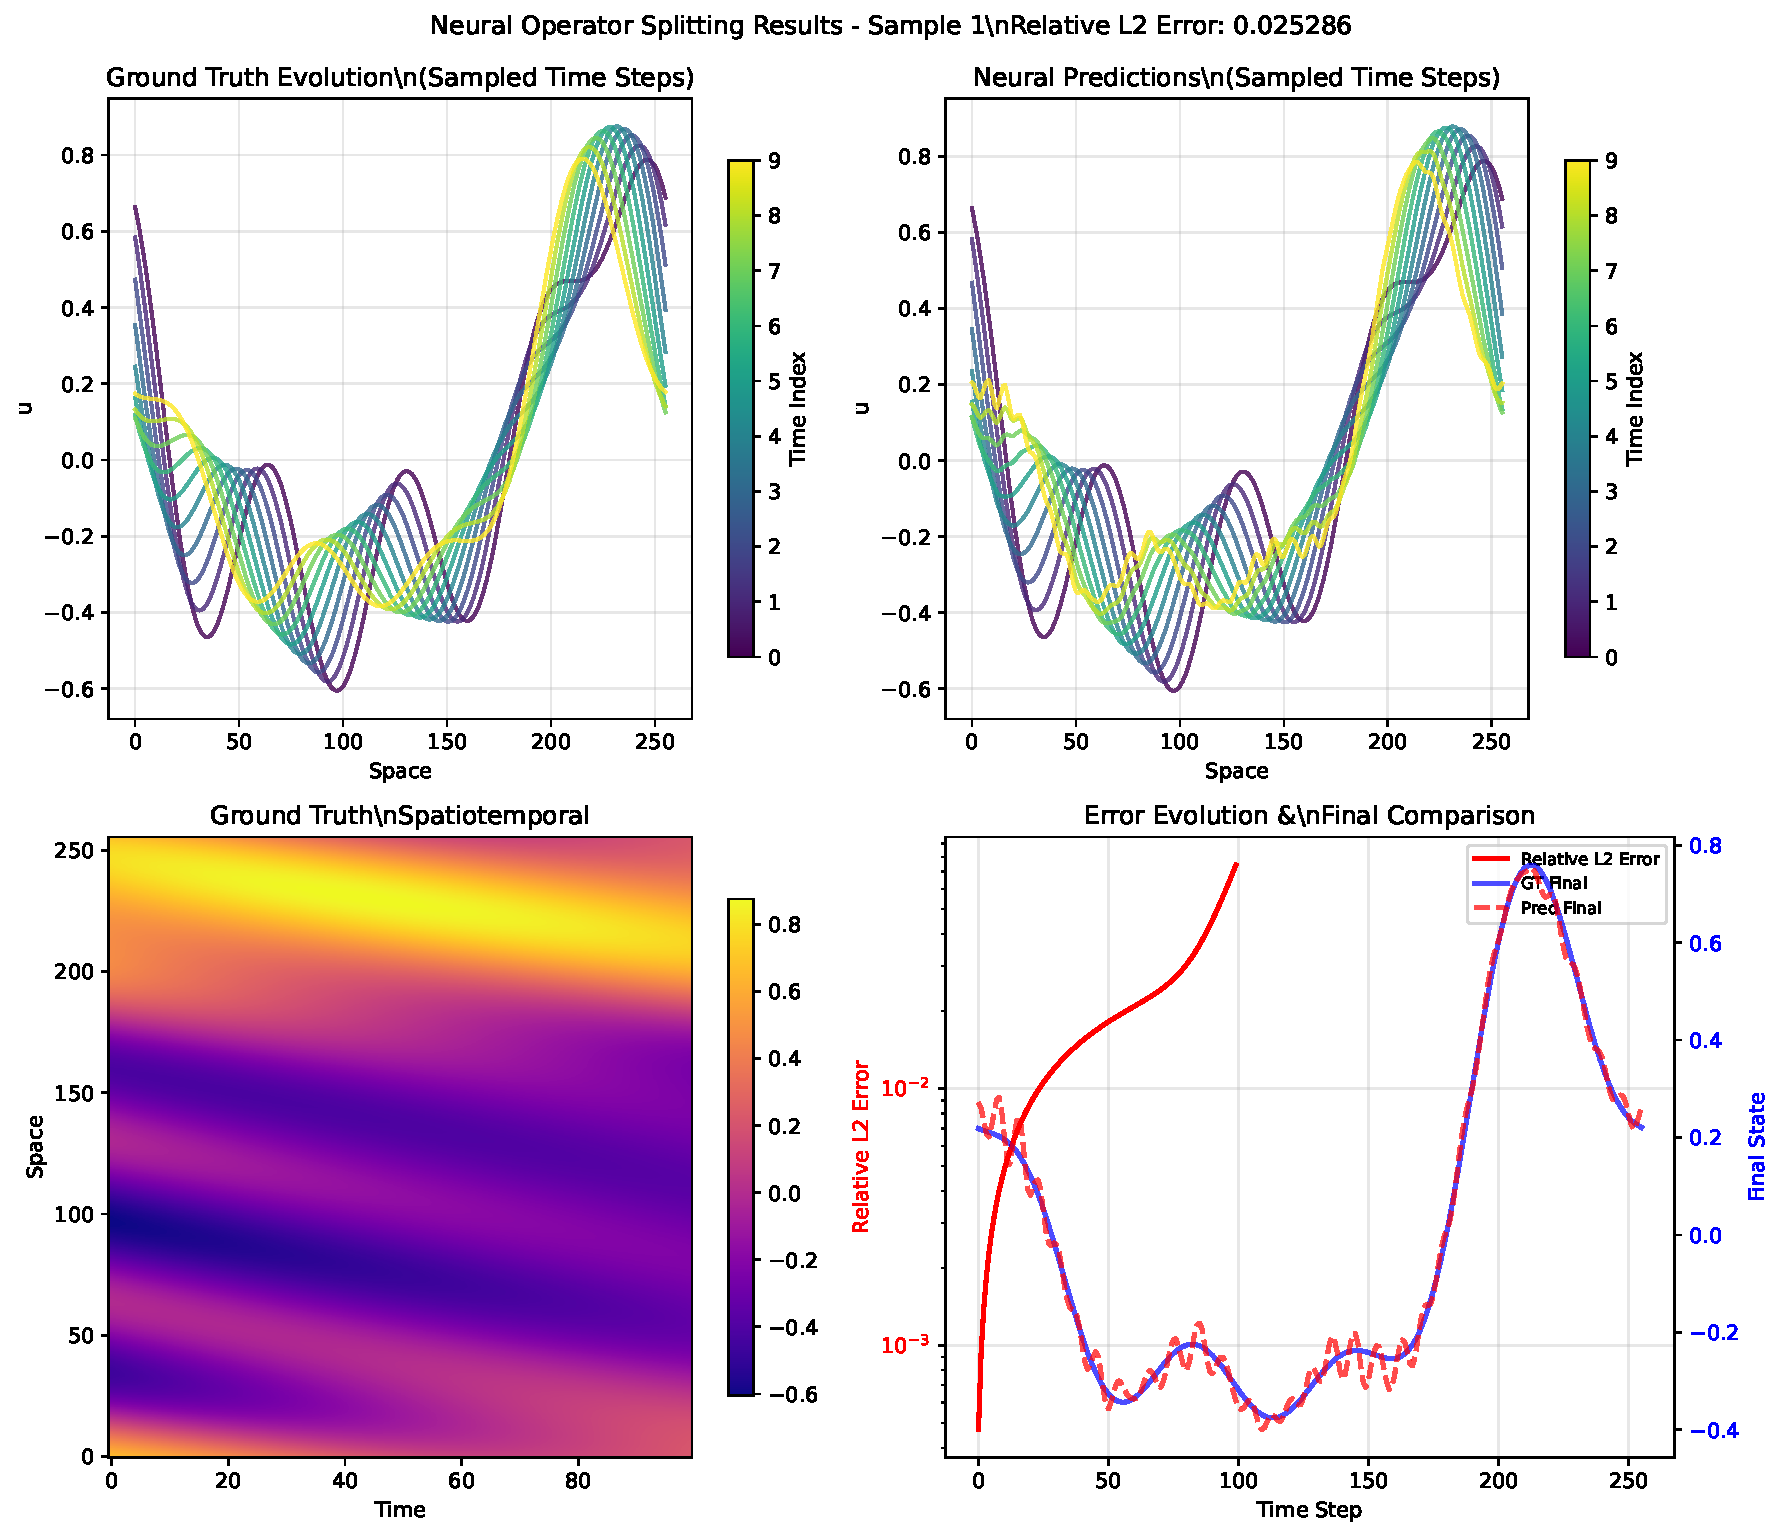
\includegraphics[width=\linewidth]{plots/E_BG_prediction_1.pdf}
\caption{
\textbf{OOD trajectory prediction on diffusion+dispersion equations.} 
We select operators using beam search and autoregressively unroll dynamics for 100 timesteps. The top panels show ground truth (left) and model predictions (right). The bottom panel displays error evolution throughout the rollout and compares the final prediction against ground truth.
}
\label{fig:diffusion+dispersion}
\end{figure}


\begin{figure}[h]
\centering
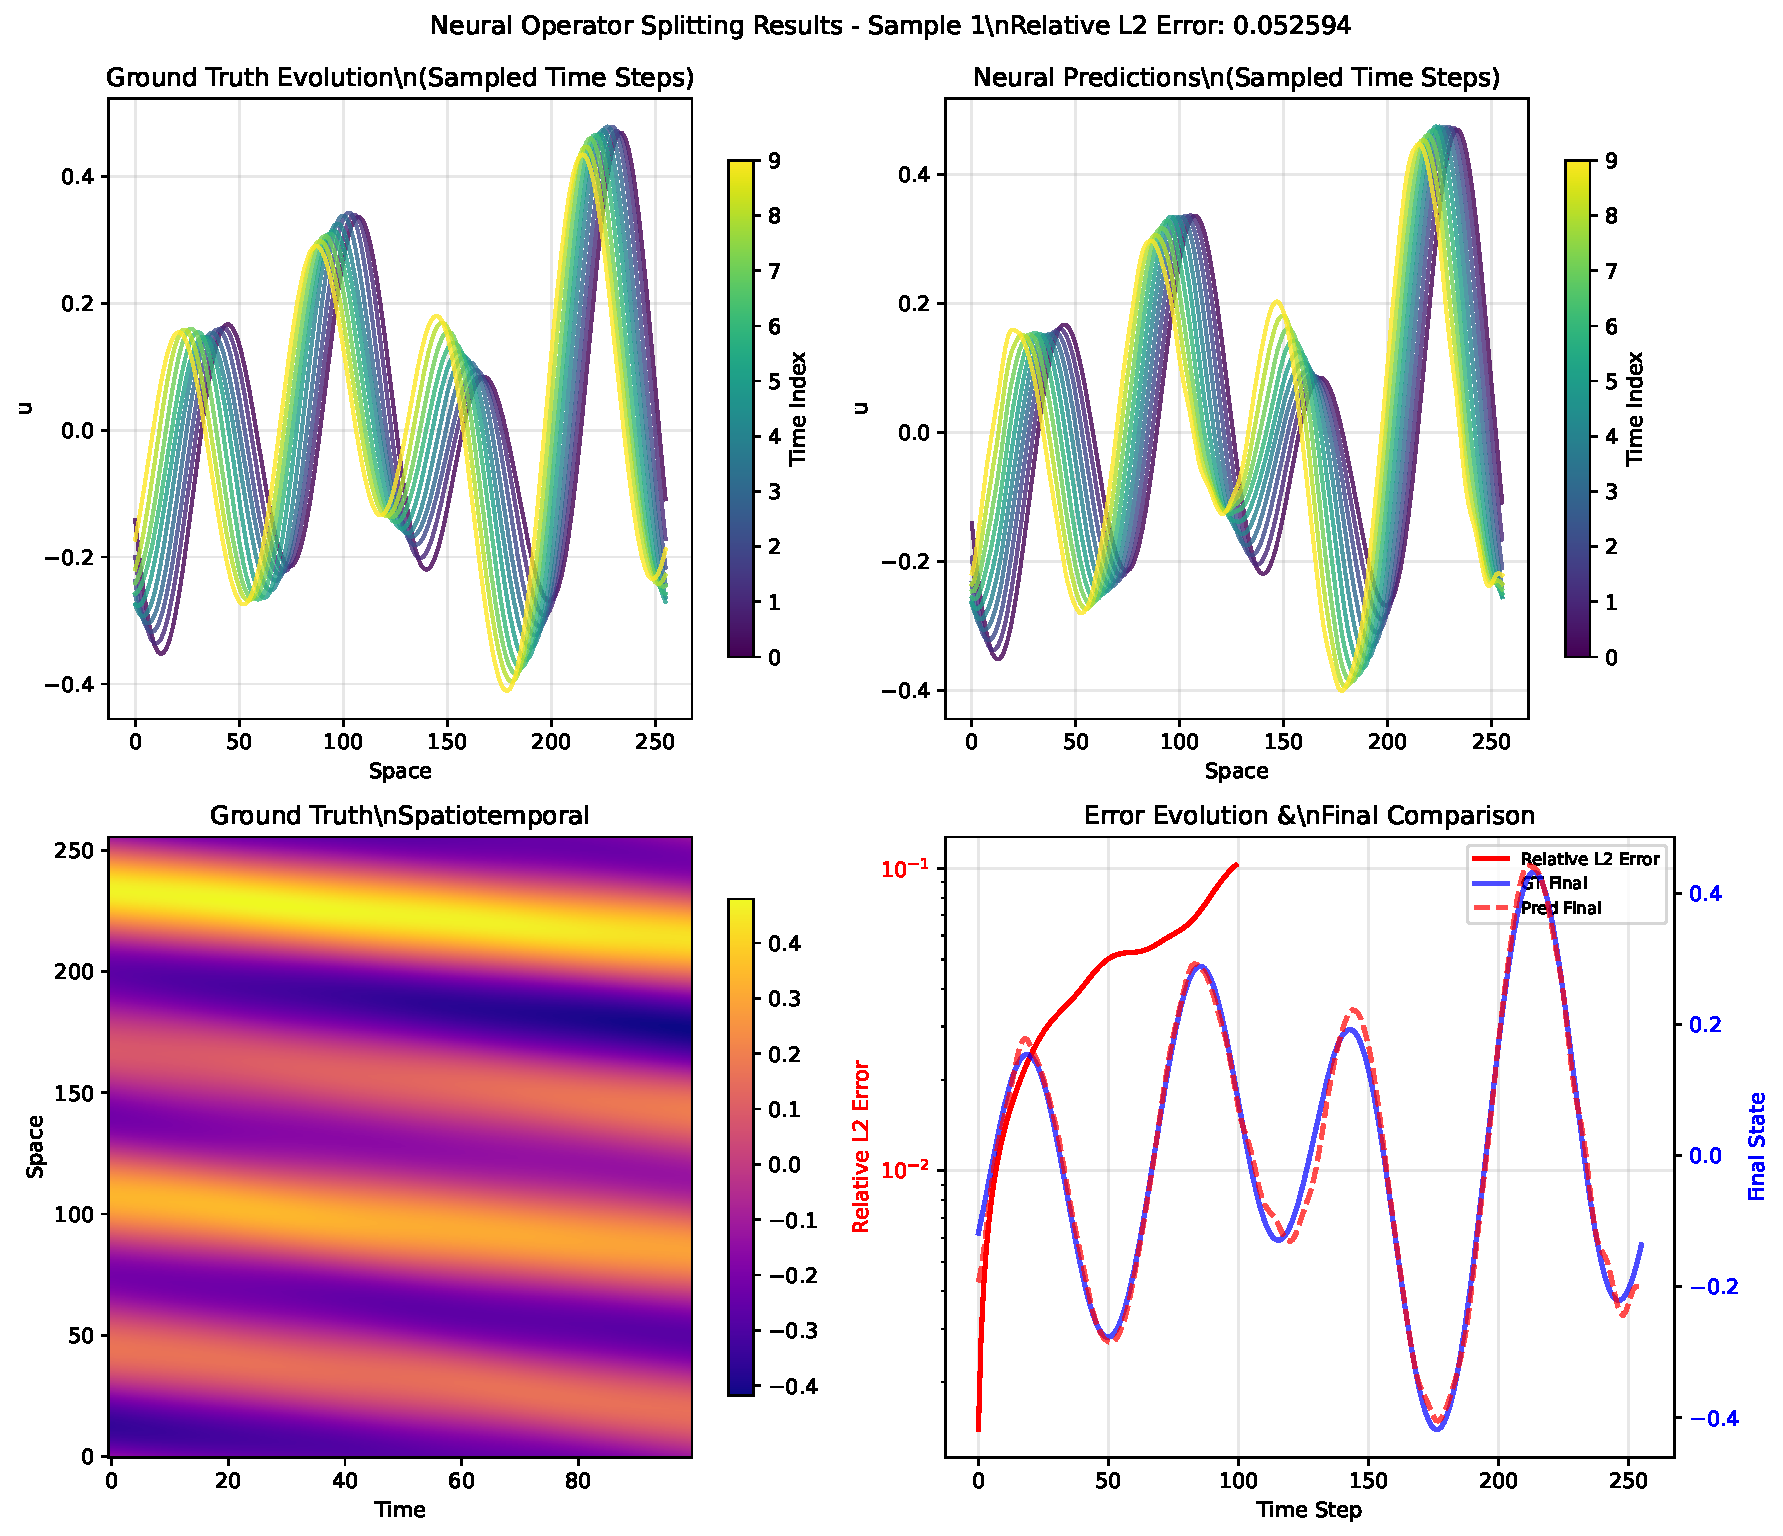
\includegraphics[width=\linewidth]{plots/E_ED_prediction_5.pdf}
\caption{
\textbf{OOD trajectory prediction on nonlinear advection+dispersion.} We select operators using beam search and autoregressively unroll dynamics for 100 timesteps. The top panels show ground truth (left) and model predictions (right). The bottom panel displays error evolution throughout the rollout and compares the final prediction against ground truth.
}
\label{fig:nonlinear+dispersion}
\end{figure}

\begin{figure}[h]
\centering
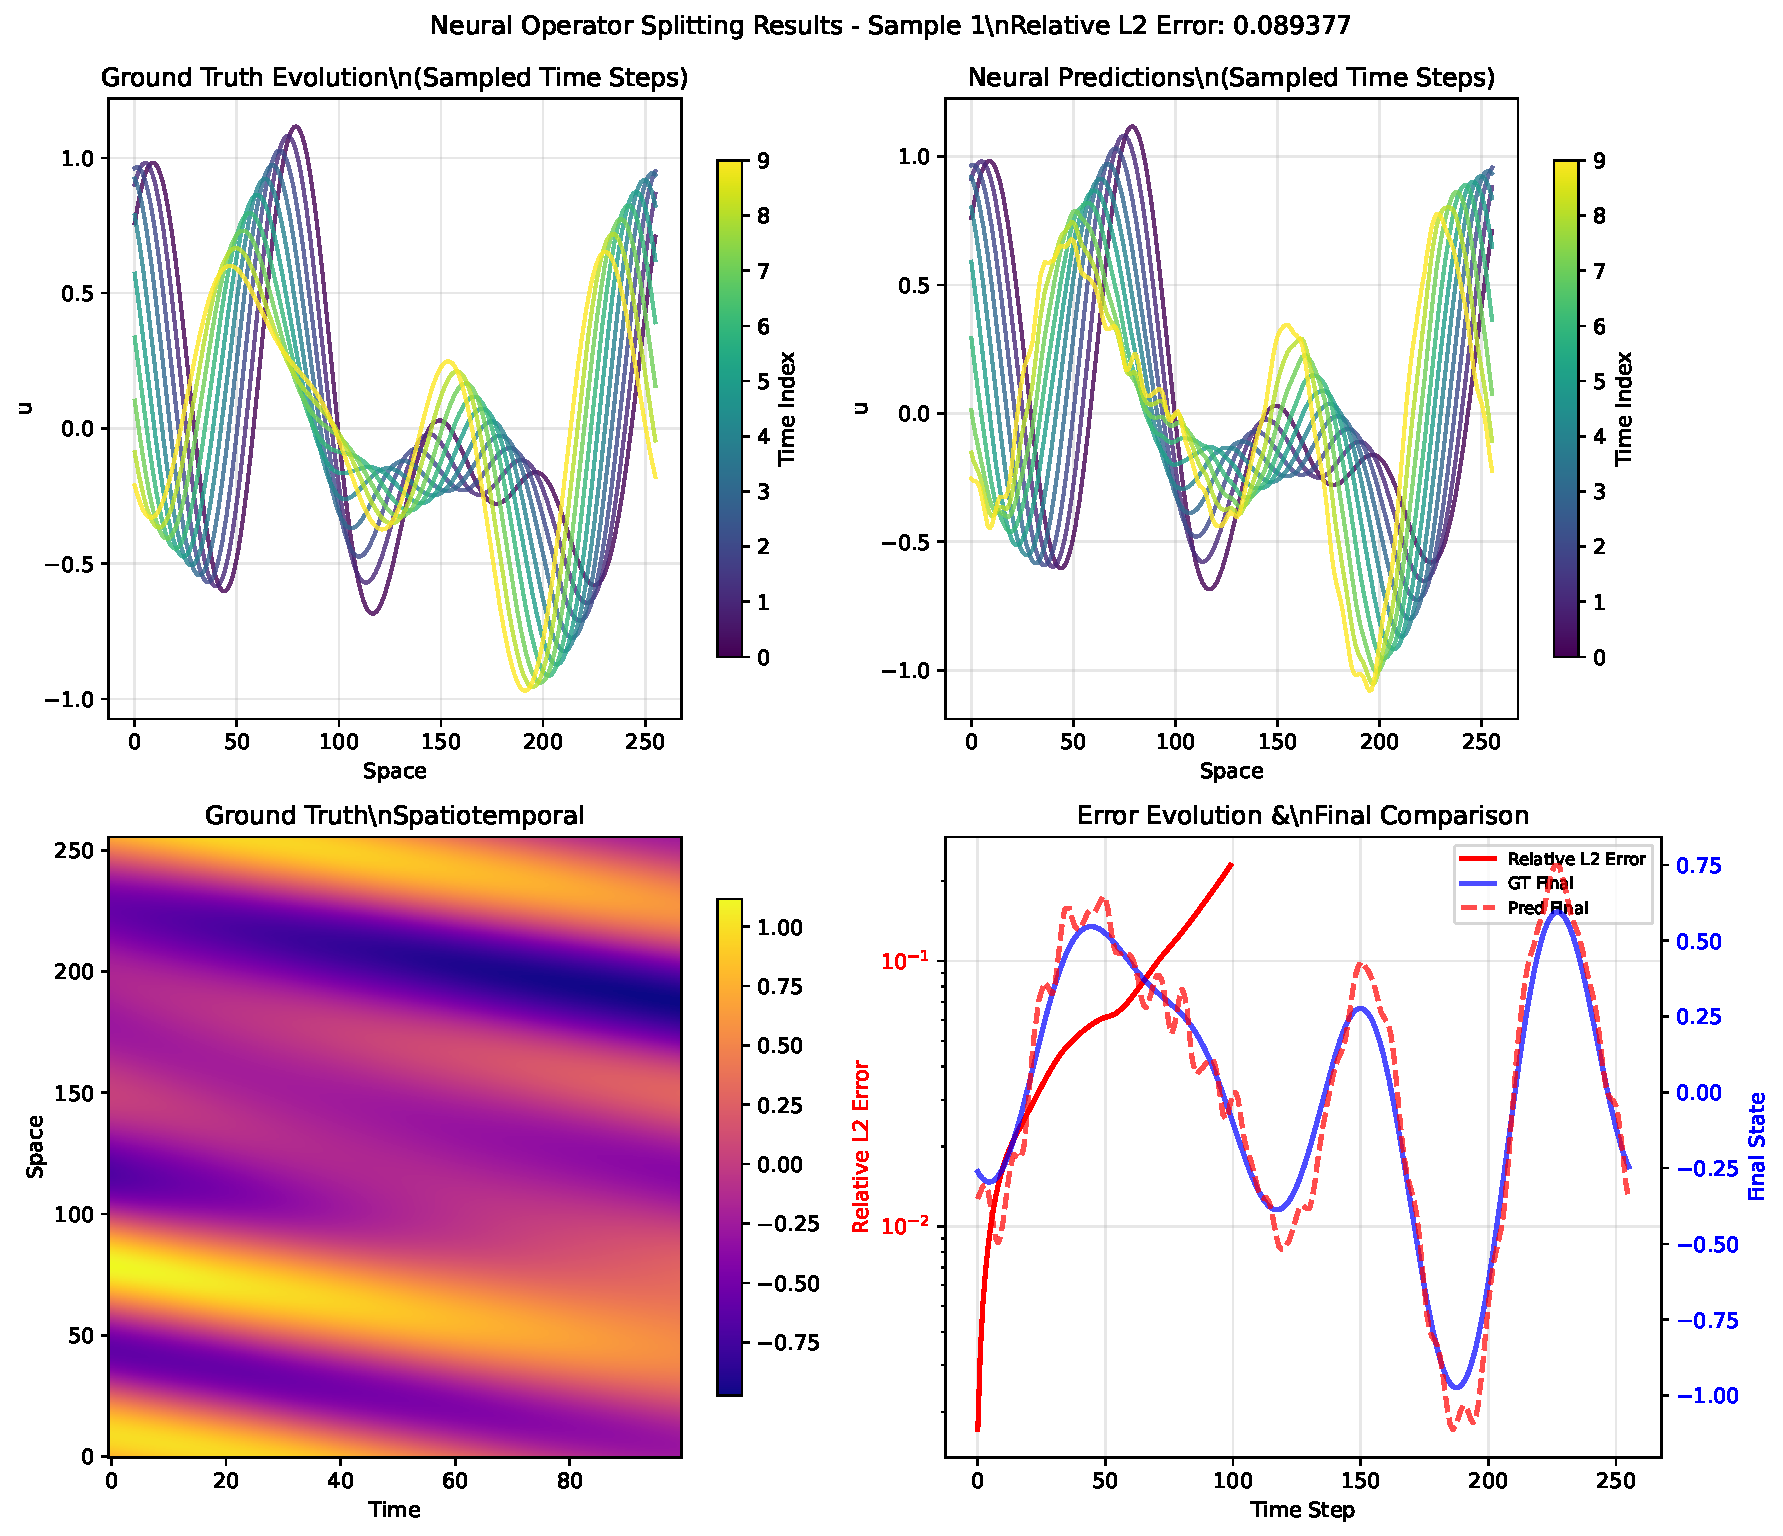
\includegraphics[width=\linewidth]{plots/E_ALL_prediction_1.pdf}
\caption{
\textbf{OOD trajectory prediction on nonlinear advection+dispersion+diffusion.} We select operators using beam search and autoregressively unroll dynamics for 100 timesteps. The top panels show ground truth (left) and model predictions (right). The bottom panel displays error evolution throughout the rollout and compares the final prediction against ground truth.
}
\label{fig:nonlinear+diffusion+dispersion}
\end{figure}


\begin{figure}[h]
\centering
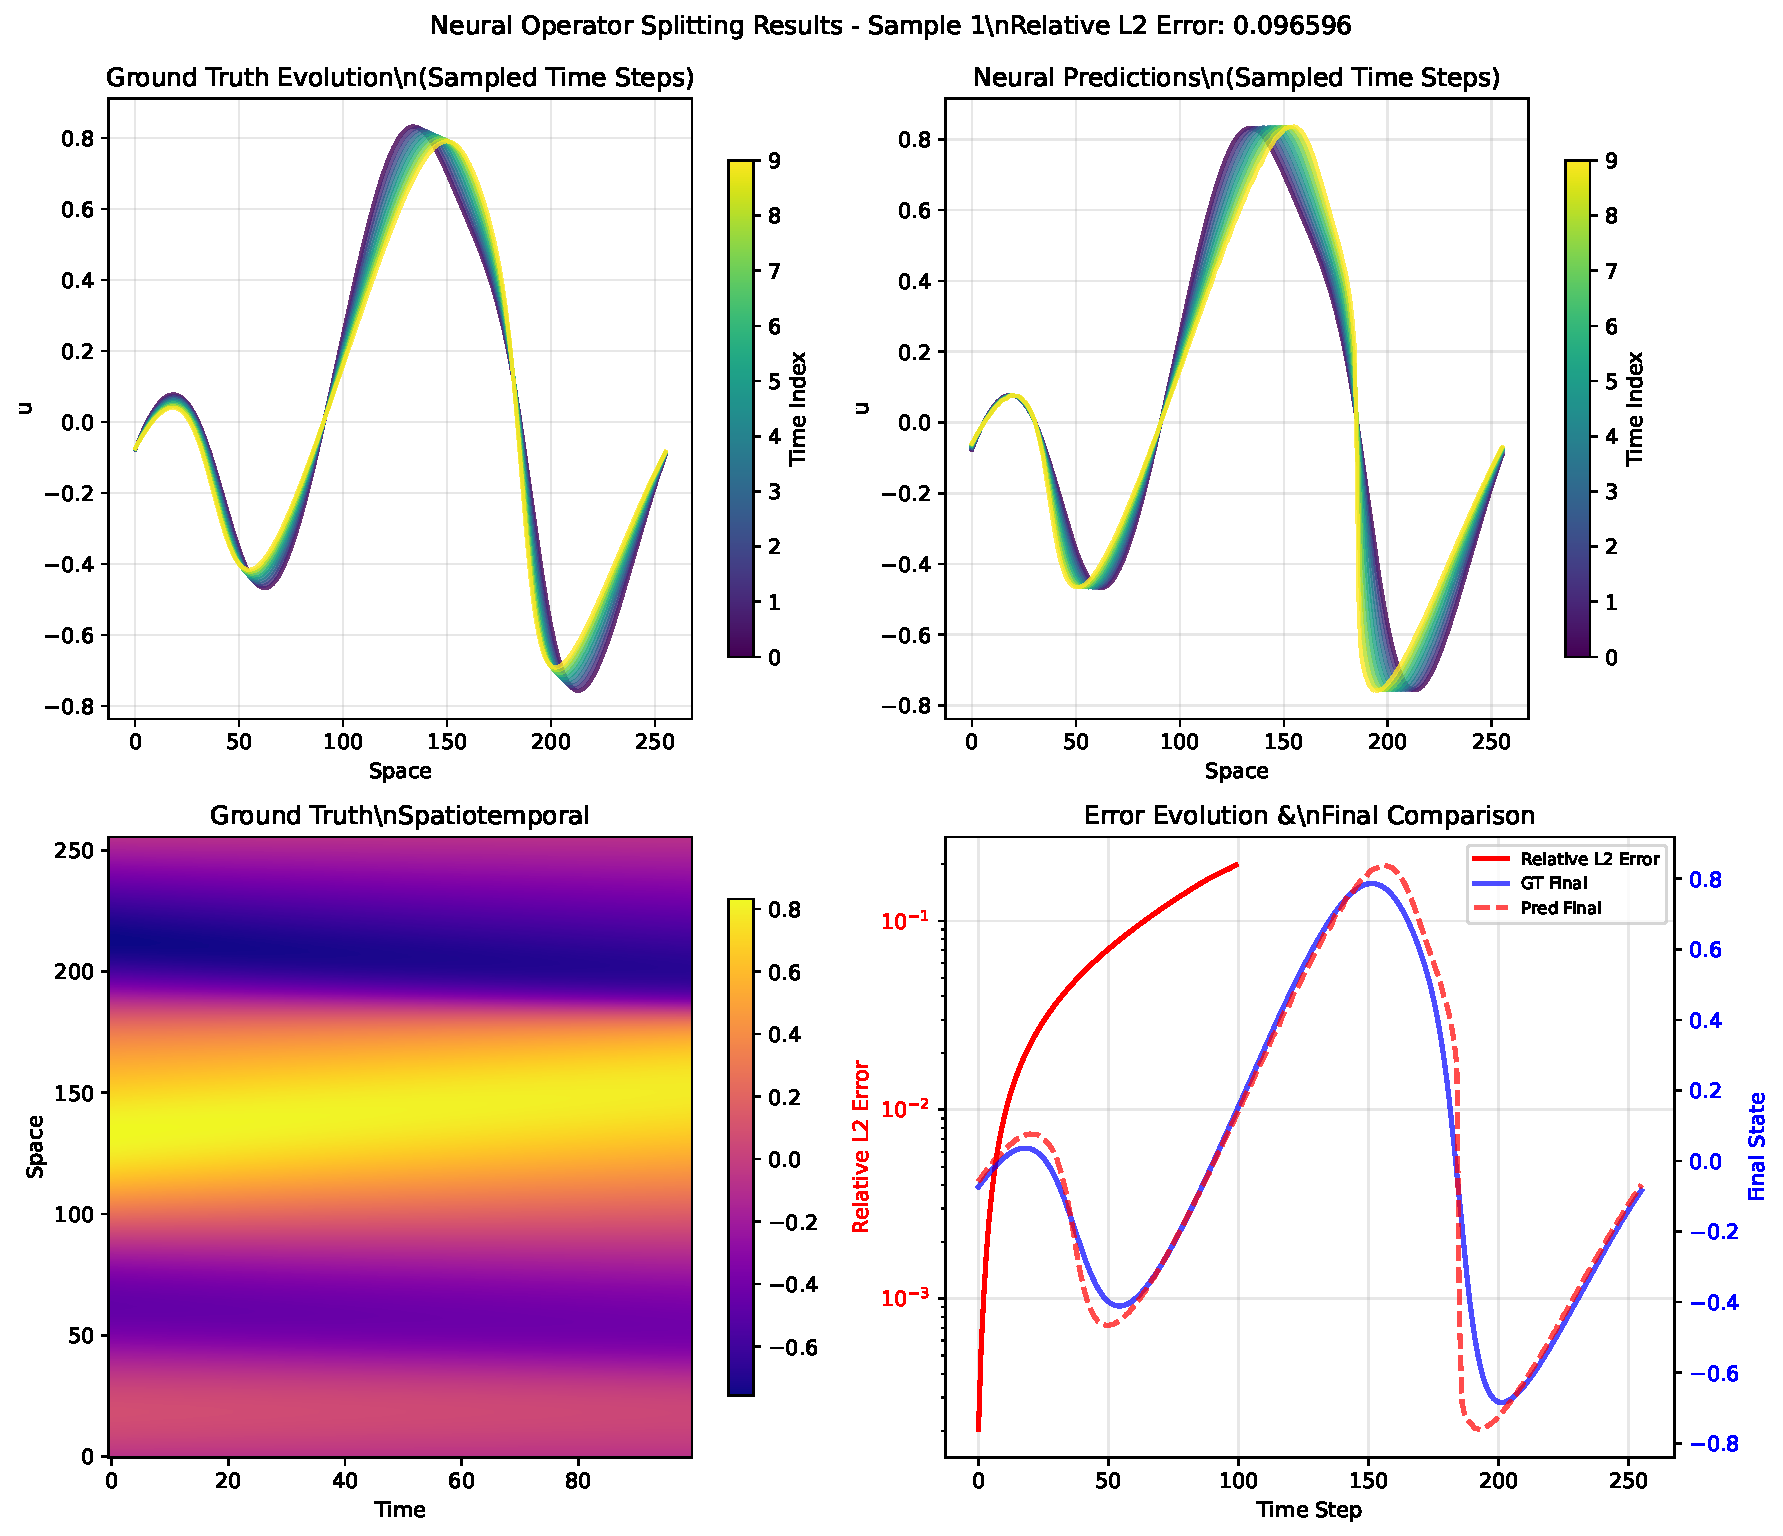
\includegraphics[width=\linewidth]{plots/E_HE_prediction_25.pdf}
\caption{
\textbf{OOD trajectory prediction on nonlinear advection+diffusion.} We select operators using beam search and autoregressively unroll dynamics for 100 timesteps. The top panels show ground truth (left) and model predictions (right). The bottom panel displays error evolution throughout the rollout and compares the final prediction against ground truth.
}
\label{fig:nonlinear+diffusion}
\end{figure}


\begin{figure}[h]
\centering
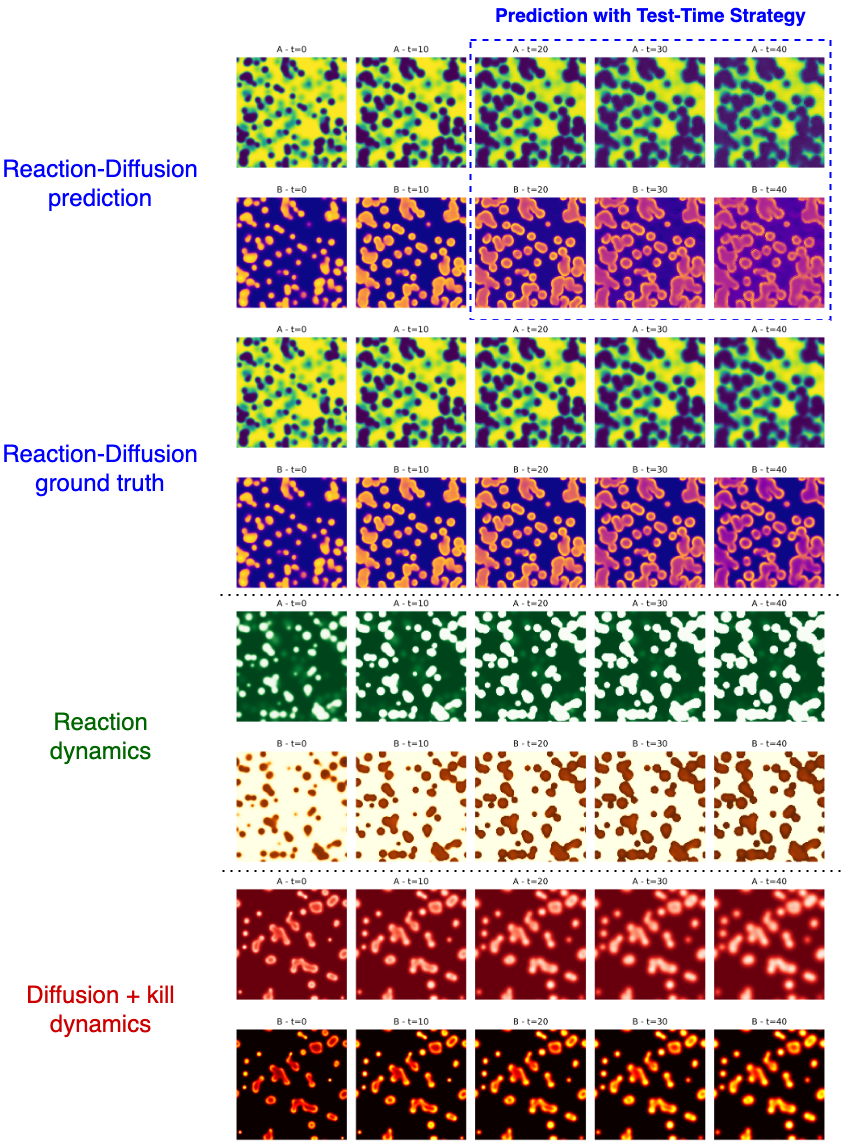
\includegraphics[width=0.8\linewidth]{plots/zero-shot-prediction-2channels.png}
\caption{
\textbf{OOD trajectory prediction on Gray--Scott equations.} 
Visualization of operator splitting decomposition for Gray--Scott reaction-diffusion dynamics. The top section compares our test-time strategy predictions (blue box) against ground truth for the full reaction-diffusion system, showing species A (yellow-green) and B (red-blue) concentrations. The bottom section displays the kind of dynamics seen during training: pure reaction terms (green/brown) and diffusion with kill terms (red/orange) for both species.}
\label{fig:zero-shot-prediction-2channels}
\end{figure}


\begin{figure}[h]
\centering
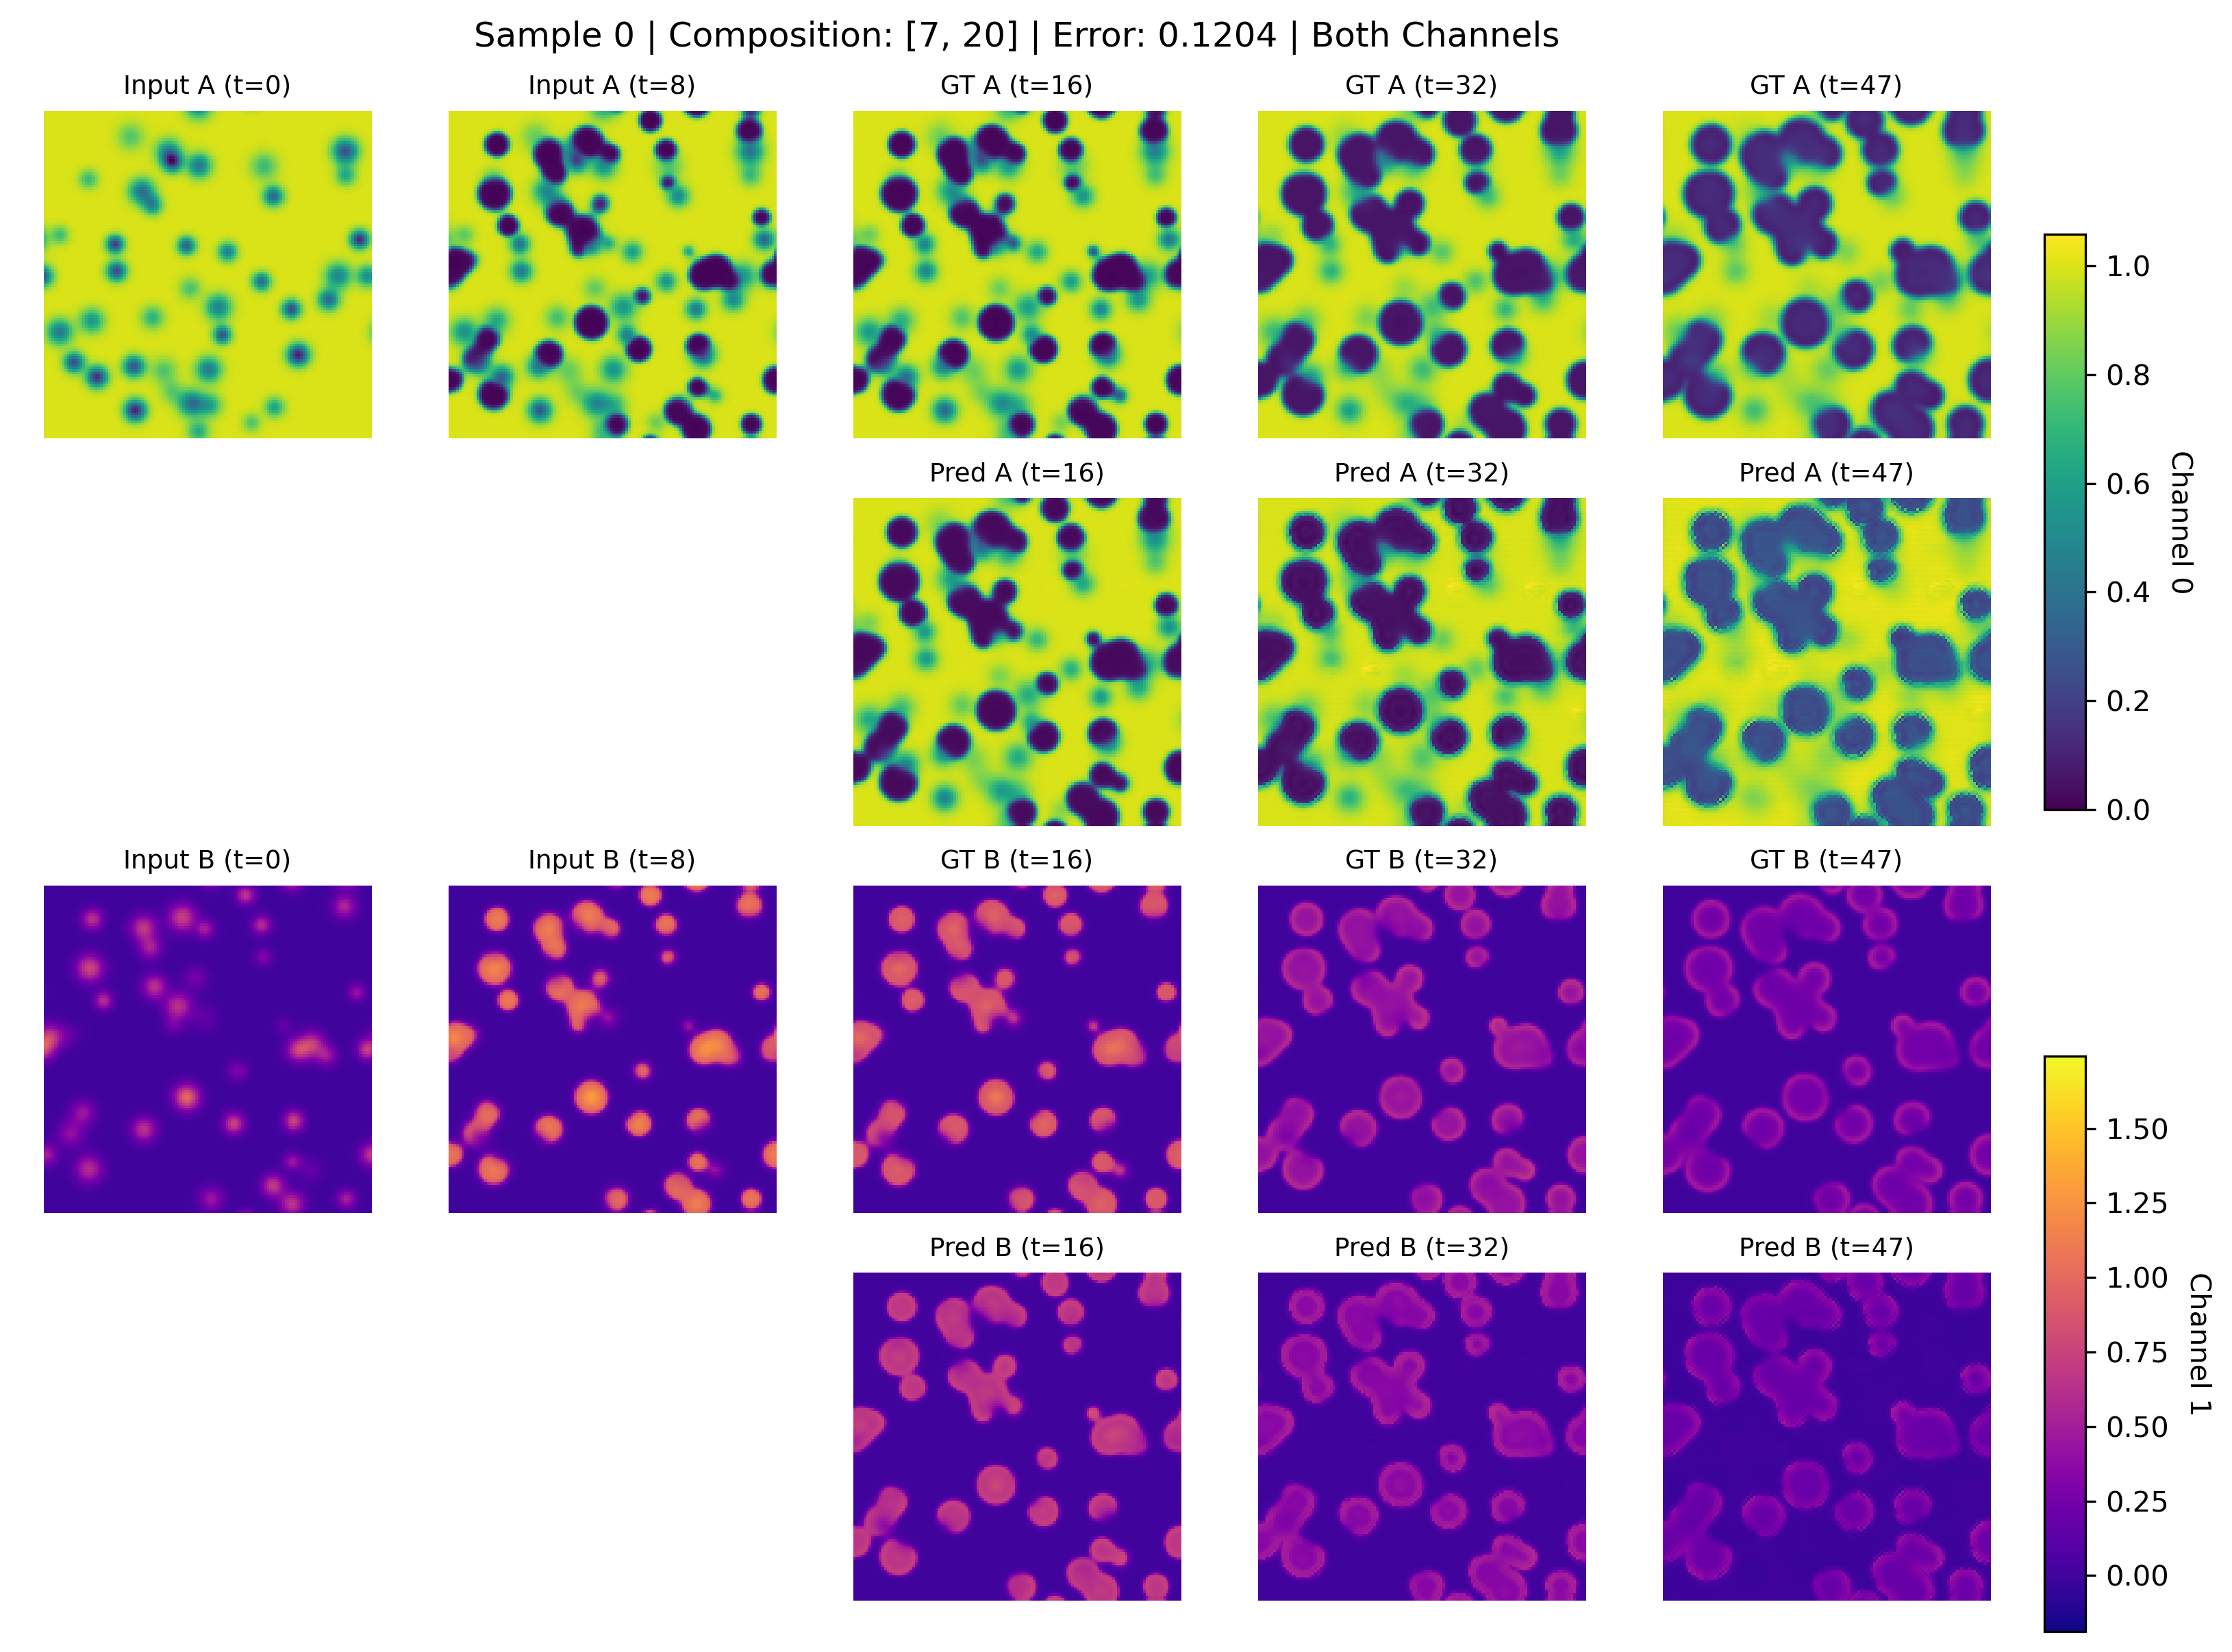
\includegraphics[width=\linewidth]{plots/sample_0000_comparison.png}
\caption{
\textbf{OOD trajectory prediction on Gray--Scott equations.} The first two rows show ground truth (top) and predicted (second) concentrations for species $A$. The bottom two rows display ground truth (third) and predicted (bottom) concentrations for species $B$.
}
\label{fig:gs-sample0}
\end{figure}

\begin{figure}[h]
\centering
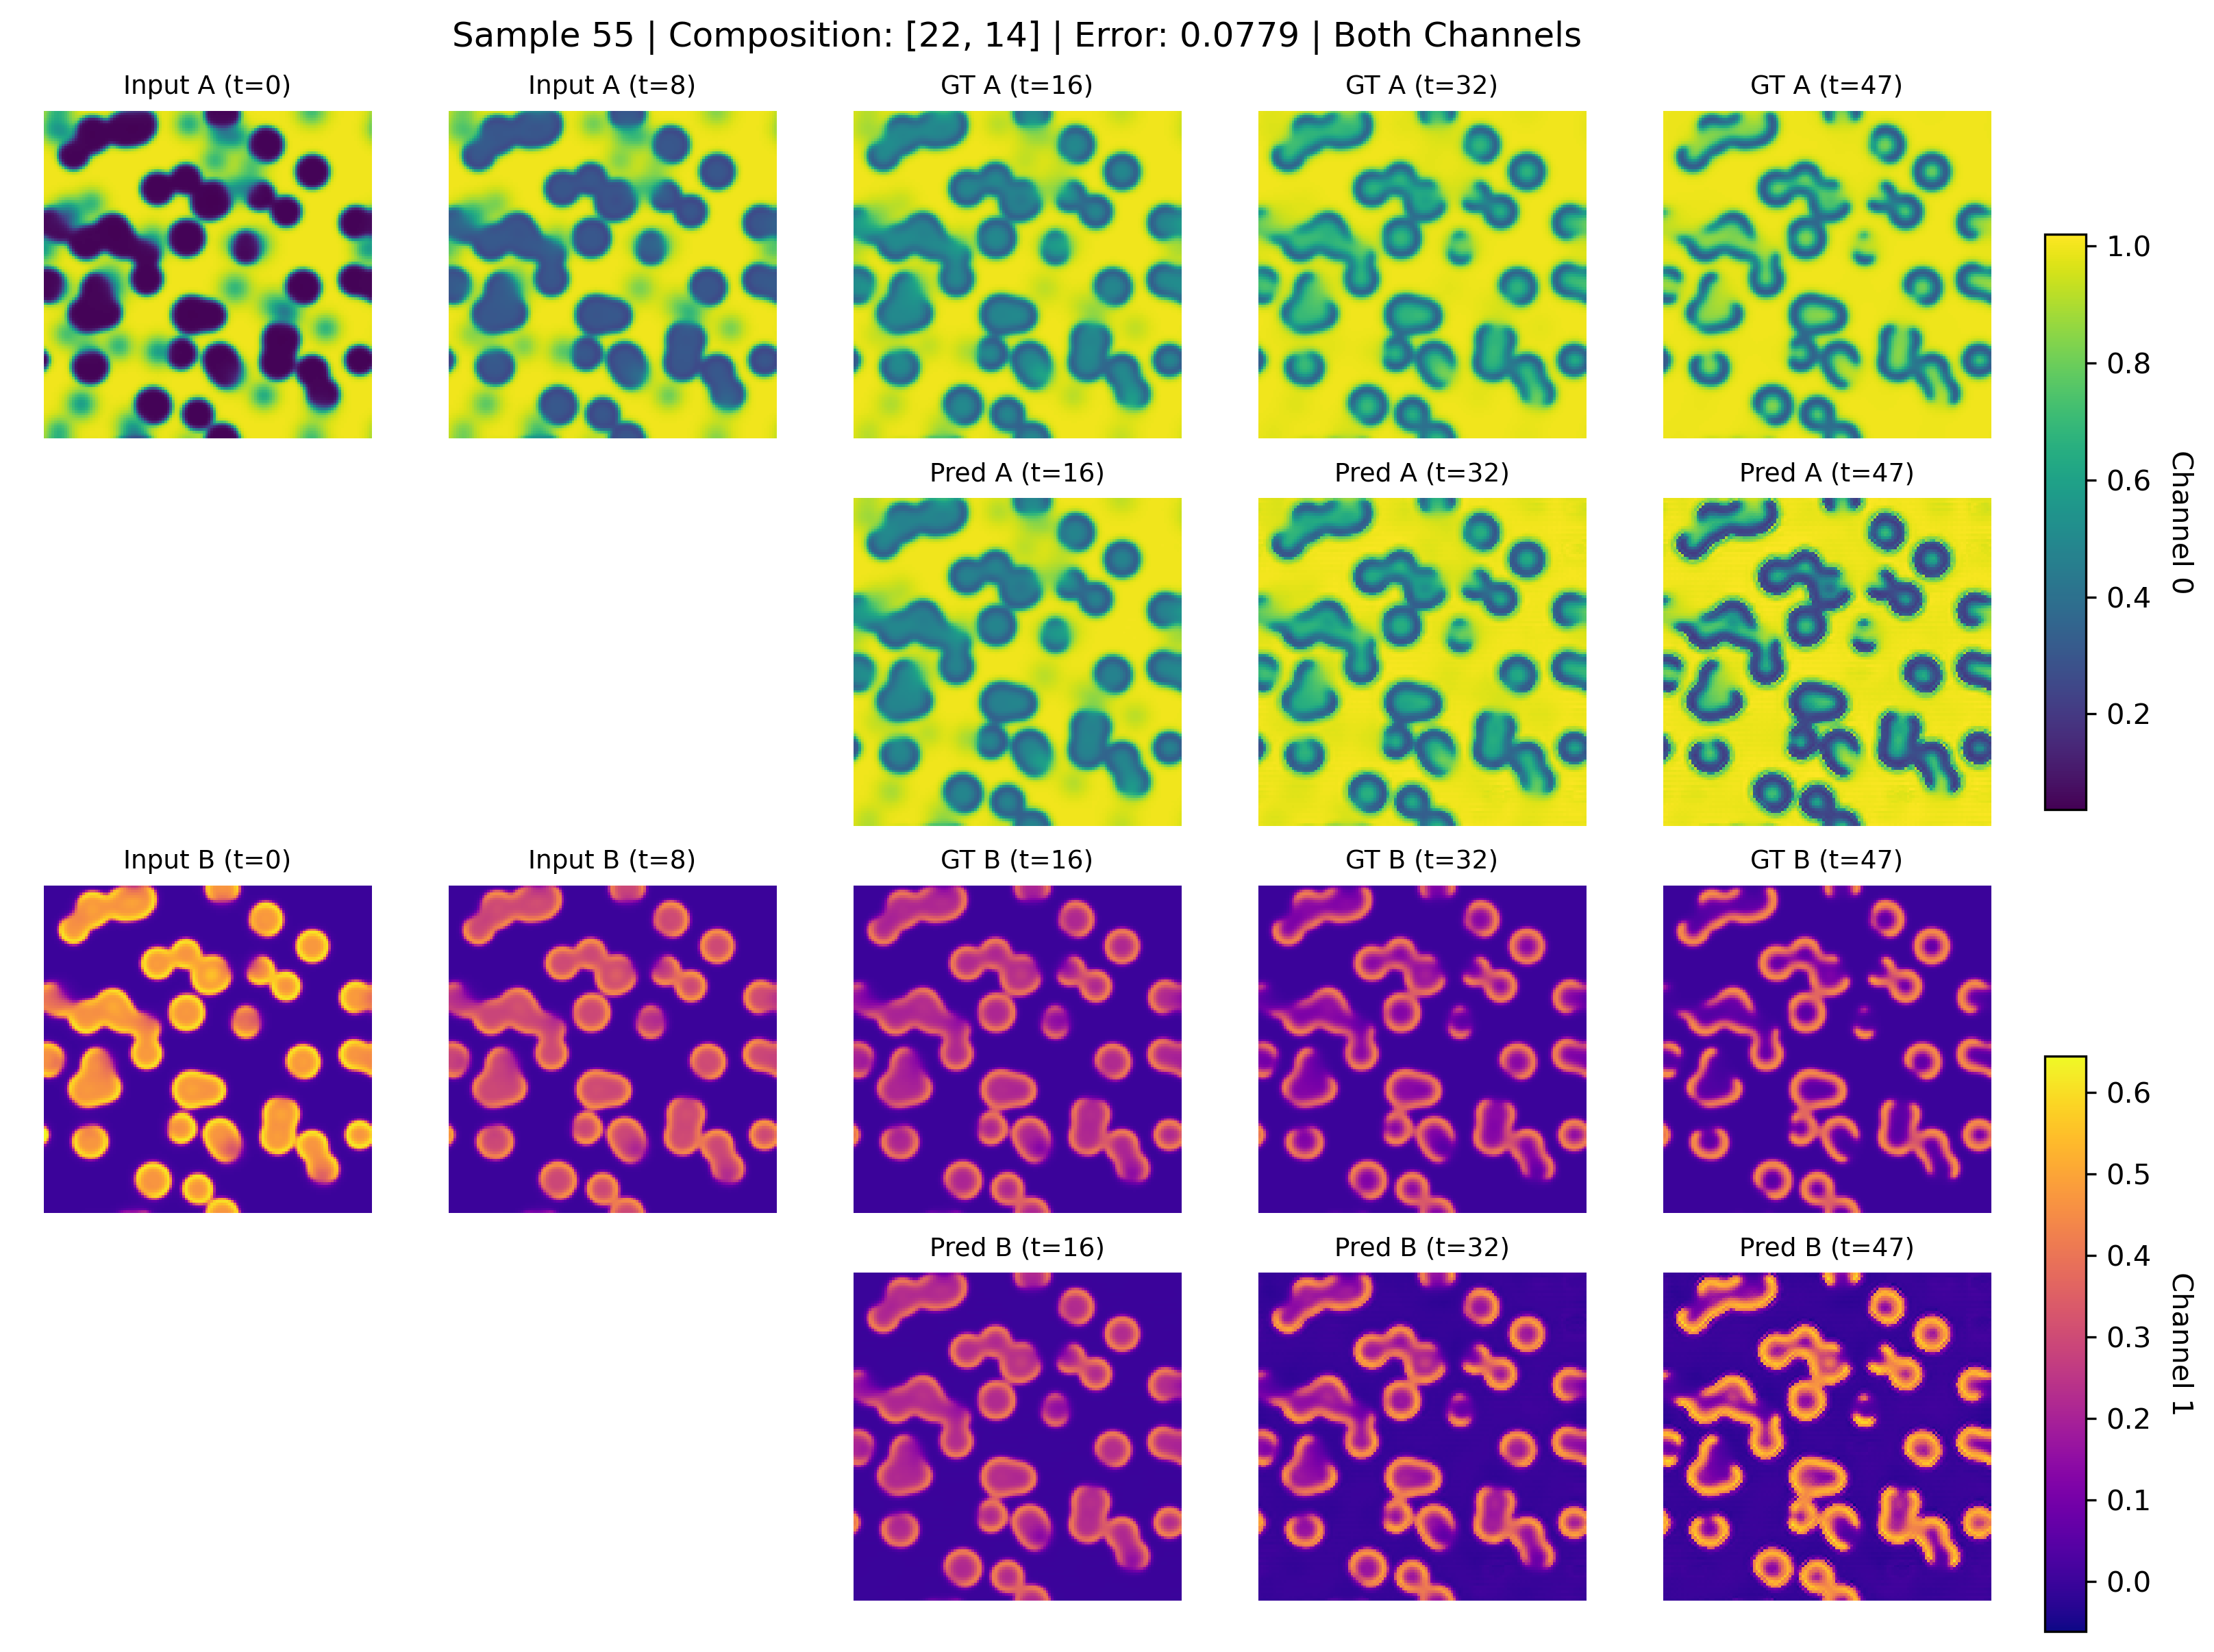
\includegraphics[width=\linewidth]{plots/sample_0055_comparison.png}
\caption{
\textbf{OOD trajectory prediction on Gray--Scott equations.} The first two rows show ground truth (top) and predicted (second) concentrations for species $A$. The bottom two rows display ground truth (third) and predicted (bottom) concentrations for species $B$.
}
\label{fig:gs-sample55}
\end{figure}

\begin{figure}[h]
\centering
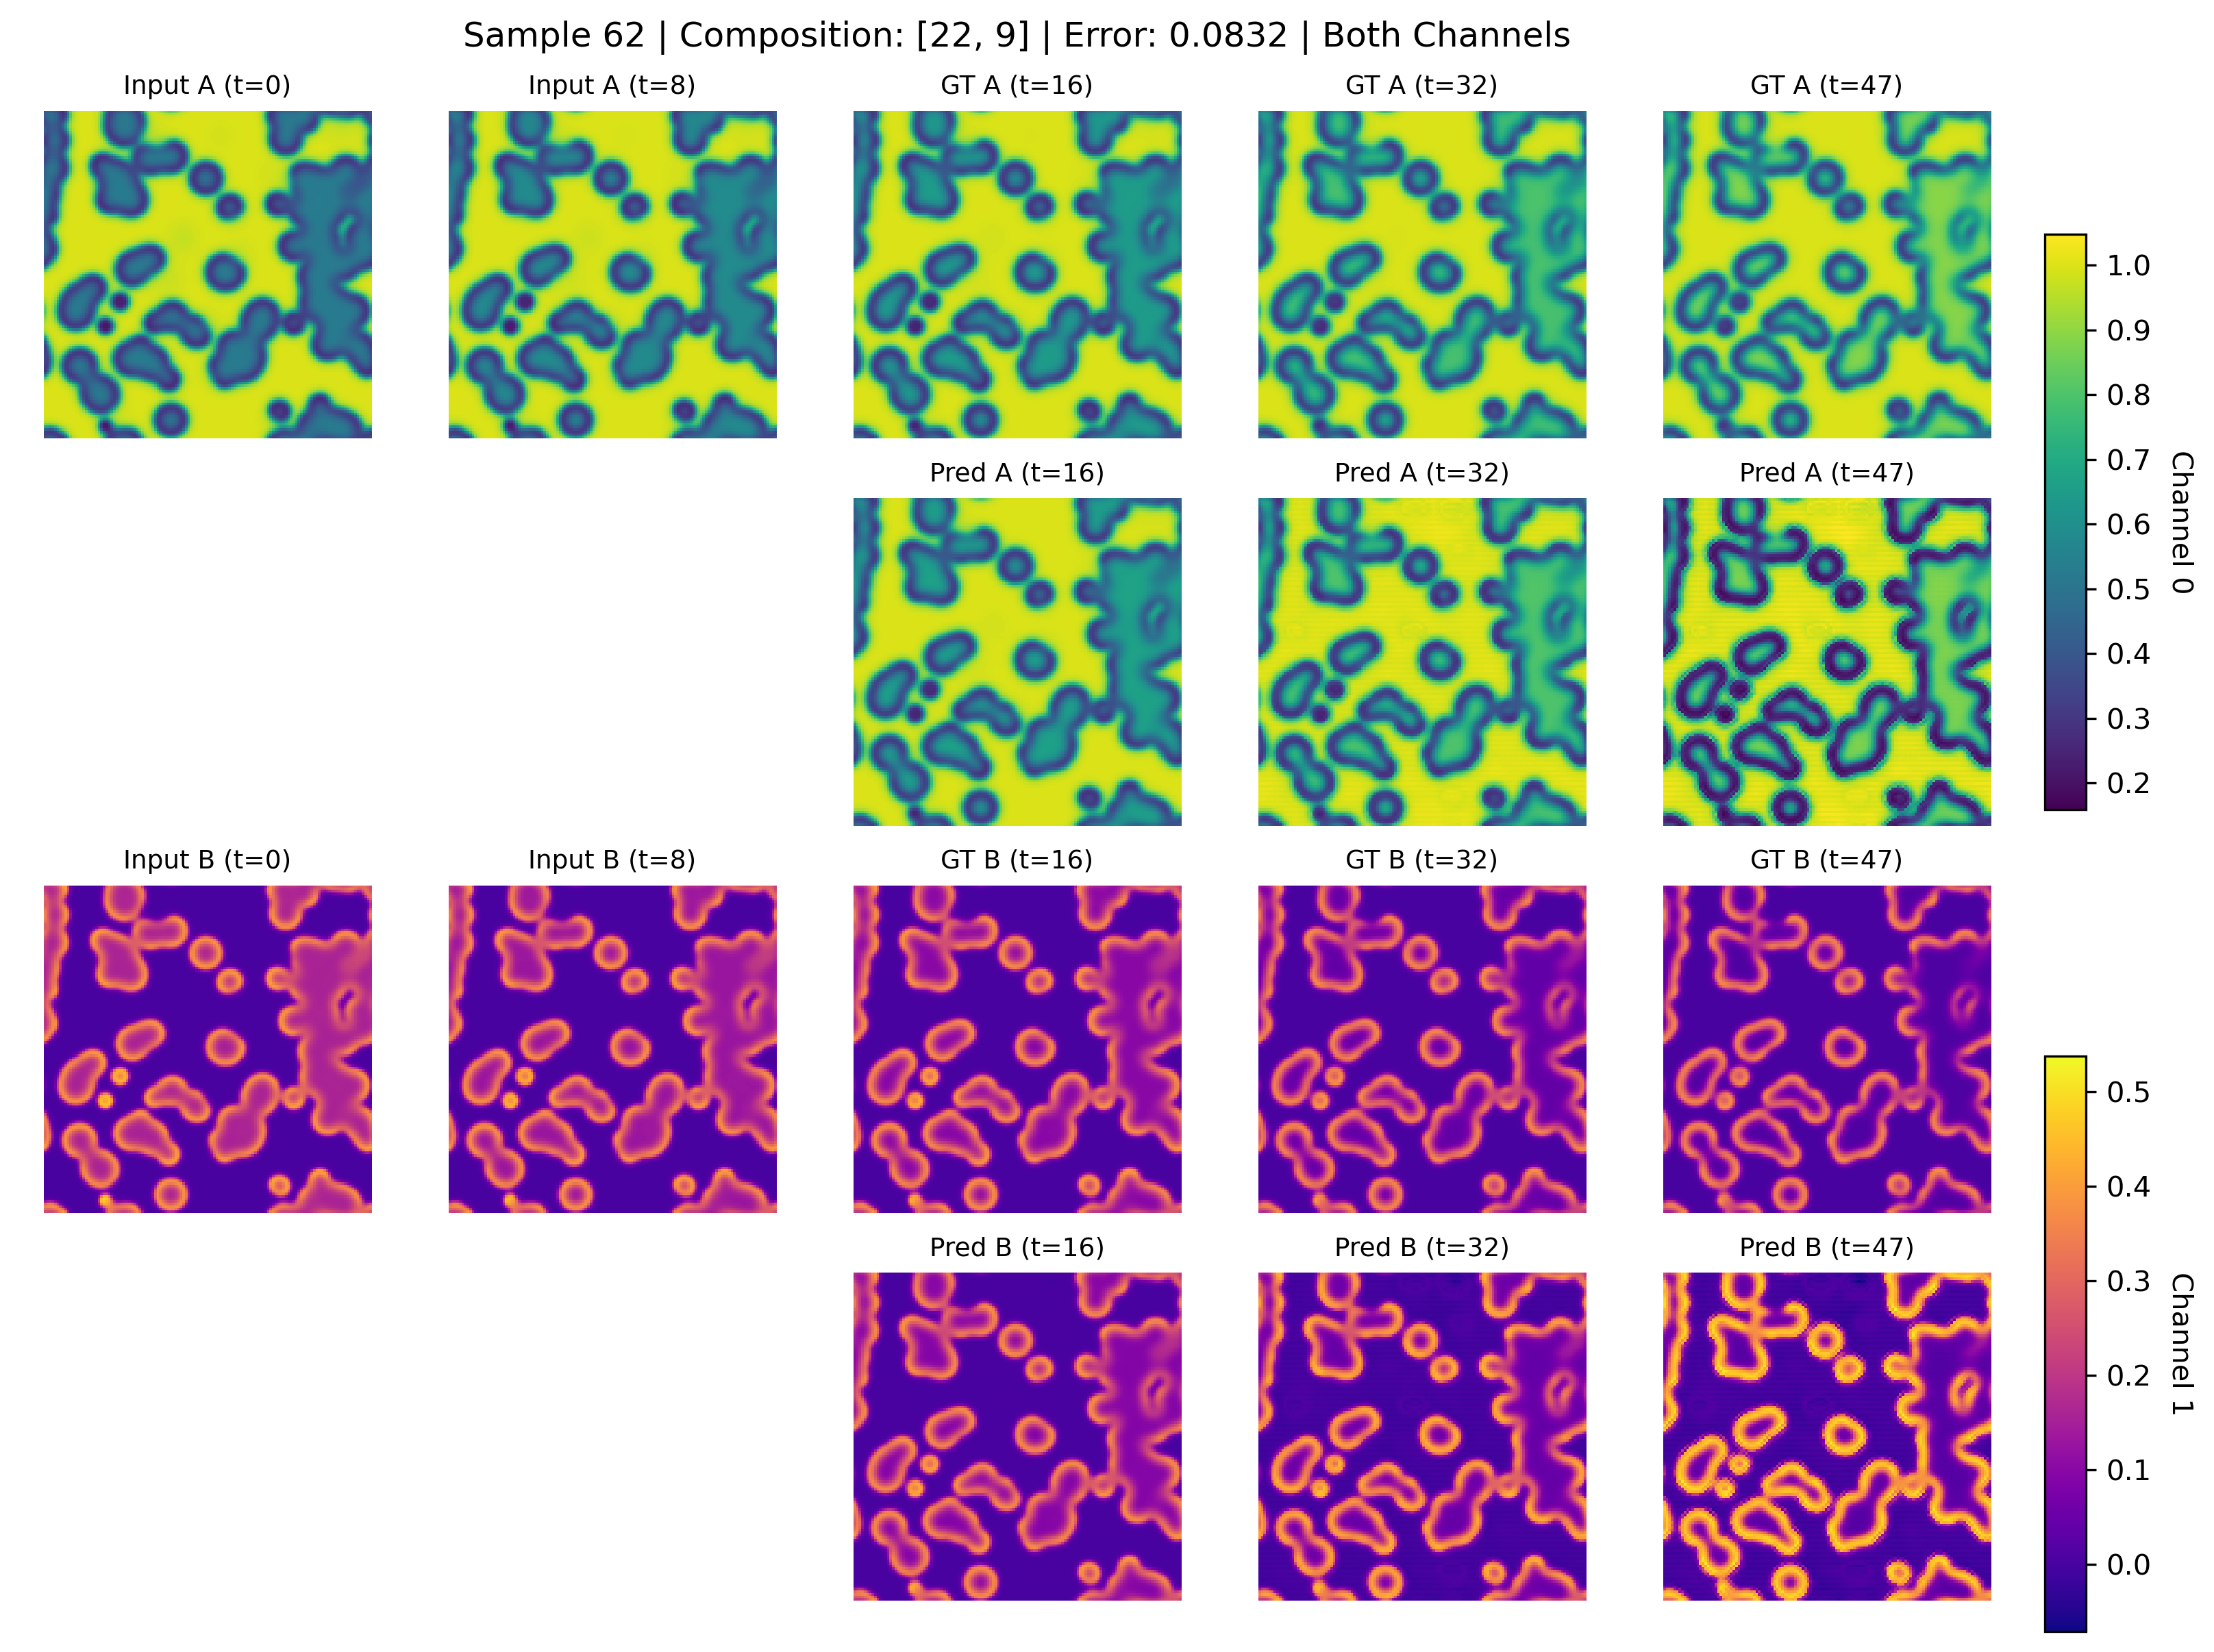
\includegraphics[width=\linewidth]{plots/sample_0062_comparison.png}
\caption{
\textbf{OOD trajectory prediction on Gray--Scott equations.} The first two rows show ground truth (top) and predicted (second) concentrations for species $A$. The bottom two rows display ground truth (third) and predicted (bottom) concentrations for species $B$.
}
\label{fig:gs-sample62}
\end{figure}

\begin{figure}[h]
\centering

\includegraphics[width=\linewidth]{plots/beam/viscosity_0.01/plot.png}
\caption{
\textbf{OOD trajectory prediction on 2D Navier--Stokes.}
Beam search composition with viscosity $\nu = 10^{-2}$.
}
\label{fig:ns-beam-1e-2}
\end{figure}

\begin{figure}[h]
\centering

\includegraphics[width=\linewidth]{plots/direct/viscosity_0.01/plot.png}
\caption{
\textbf{OOD trajectory prediction on 2D Navier--Stokes.}
Direct DISCO prediction with viscosity $\nu = 10^{-2}$.
}
\label{fig:ns-direct-1e-2}
\end{figure}

\begin{figure}[h]
\centering
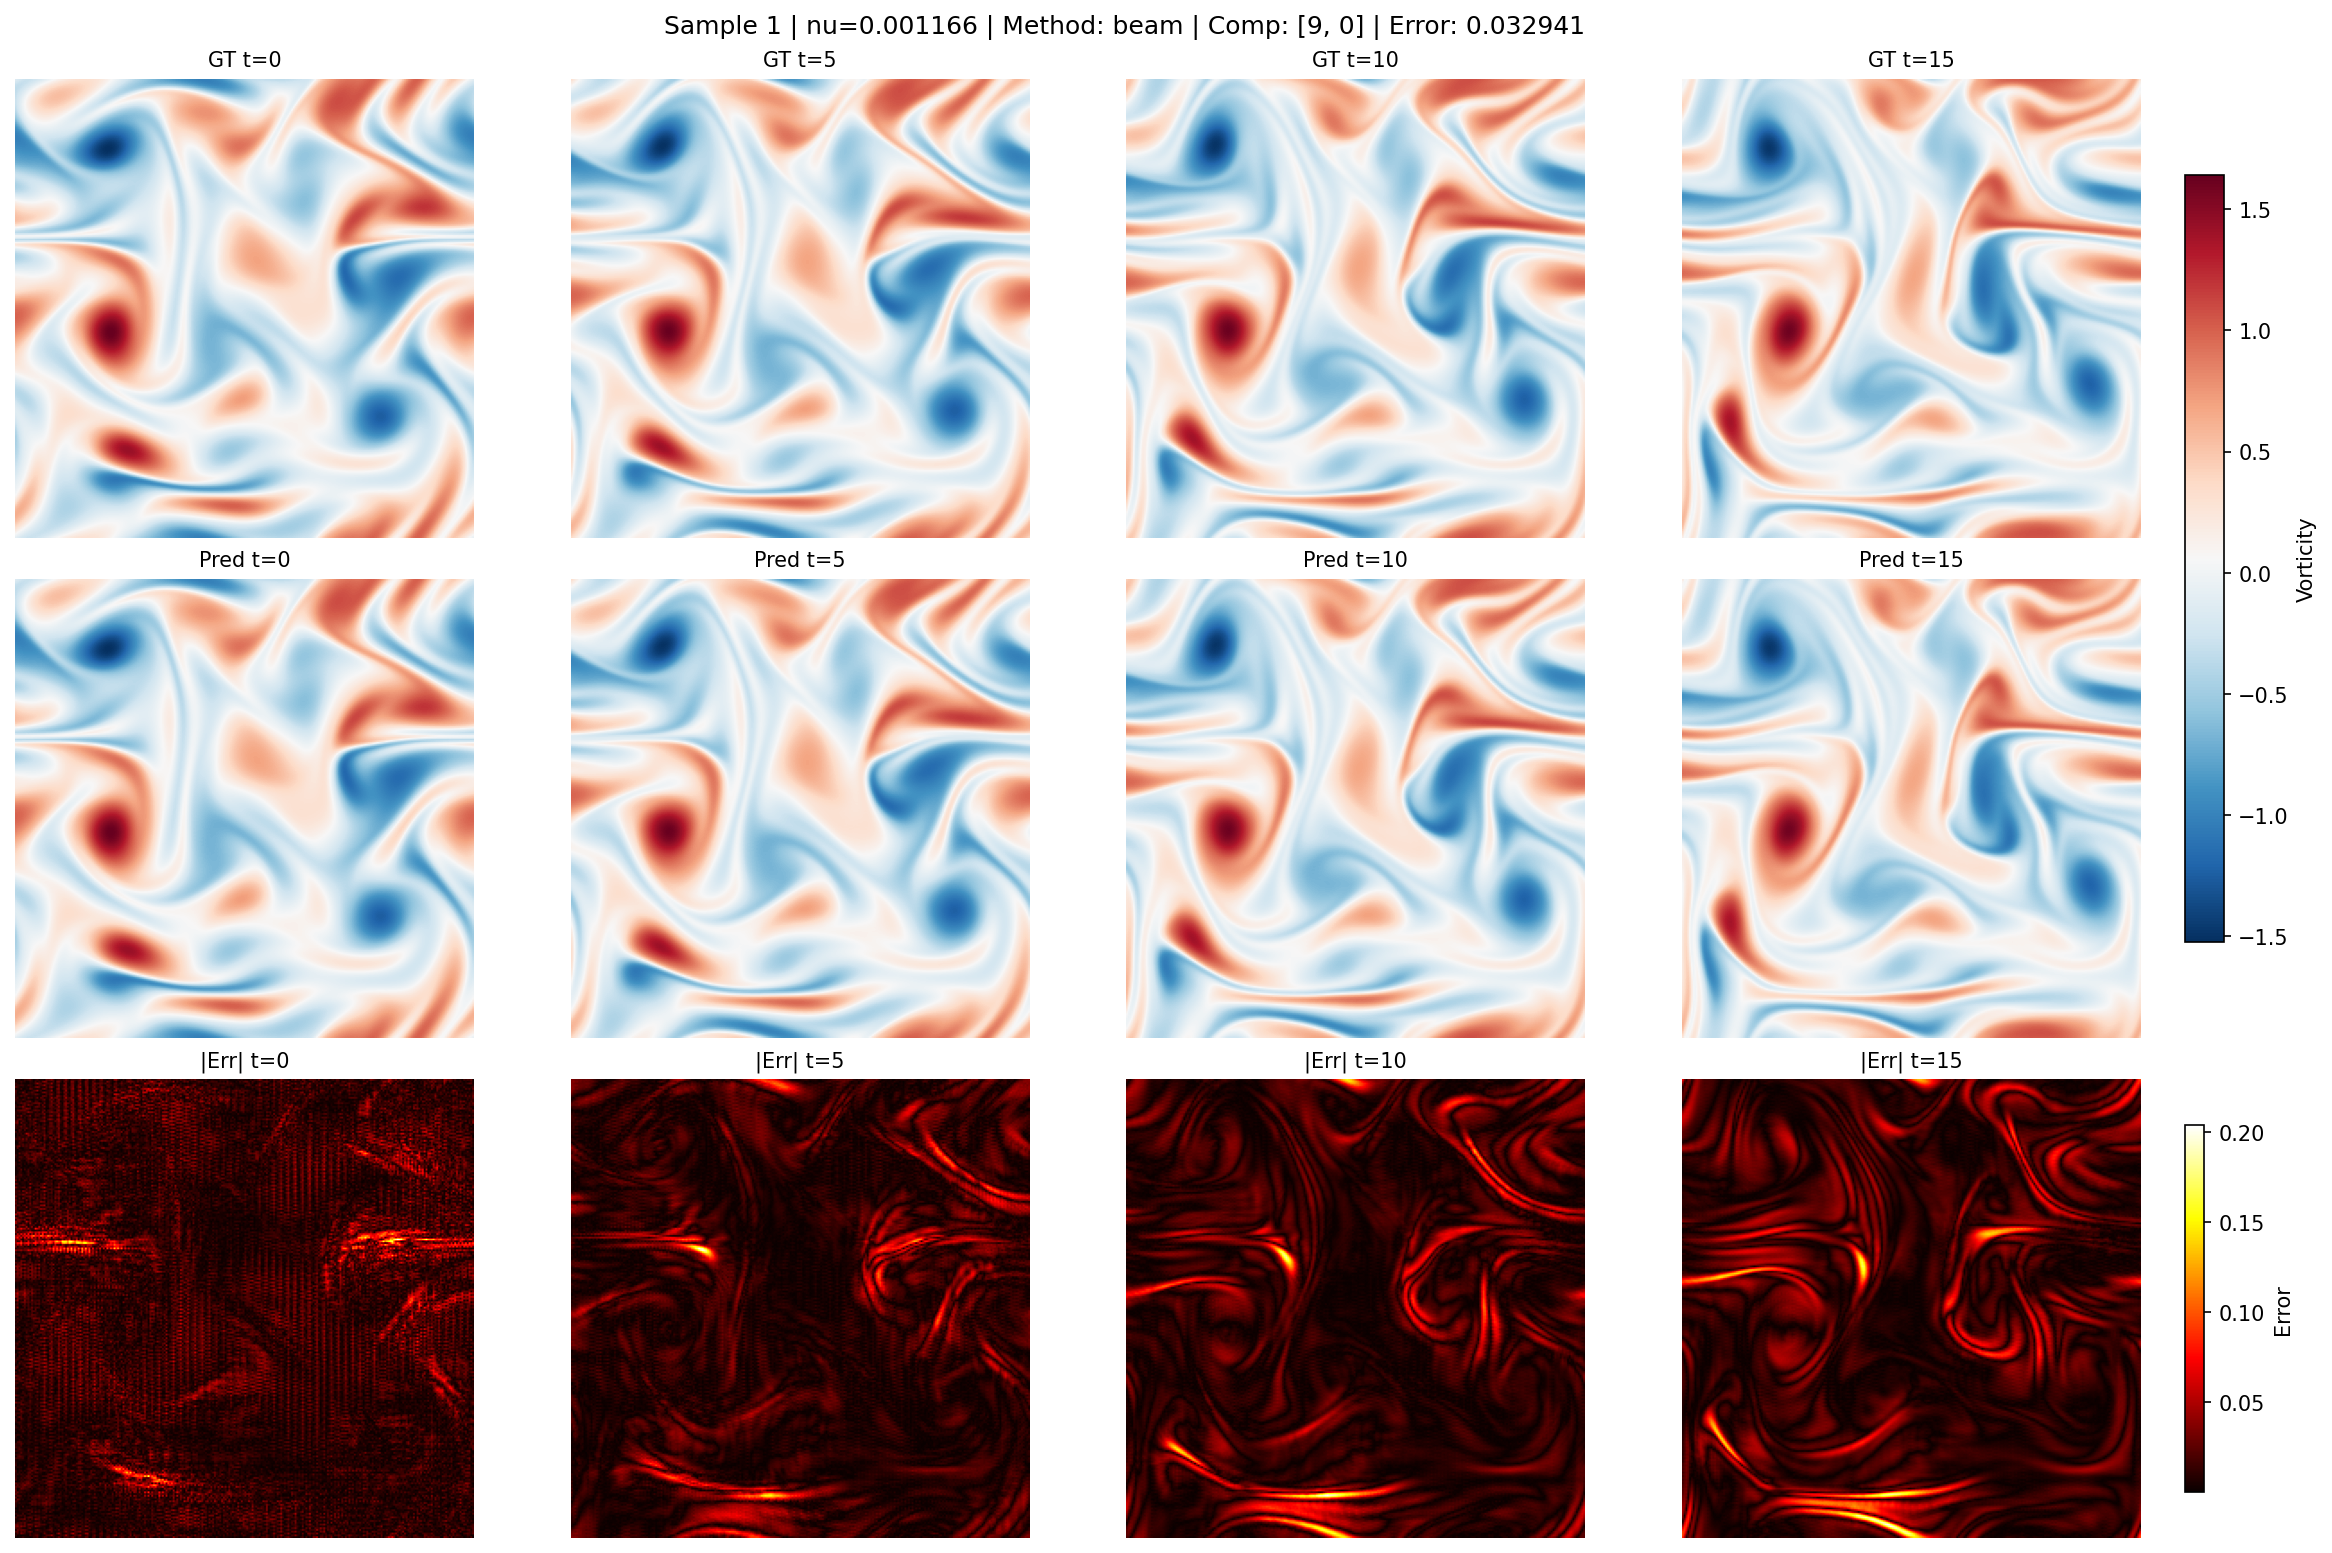
\includegraphics[width=\linewidth]{plots/beam/viscosity_0.001/plot.png}
\caption{
\textbf{OOD trajectory prediction on 2D Navier--Stokes.}
Beam search composition with viscosity $\nu = 10^{-3}$.
}
\label{fig:ns-beam-1e-3}
\end{figure}


\begin{figure}[h]
\centering

\includegraphics[width=\linewidth]{plots/direct/viscosity_0.001/plot.png}
\caption{
\textbf{OOD trajectory prediction on 2D Navier--Stokes.}
Direct DISCO prediction with viscosity $\nu = 10^{-3}$.
}
\label{fig:ns-direct-1e-3}
\end{figure}


%%%%%%%%%%%%%%%%%%%%%%%%%%%%%%%%%%%%%%%%%%%%%%%%%%%%%%%%%%%%%%%%%%%%%%%%%%%%%%%
%%%%%%%%%%%%%%%%%%%%%%%%%%%%%%%%%%%%%%%%%%%%%%%%%%%%%%%%%%%%%%%%%%%%%%%%%%%%%%%

\end{document}

% This document was modified from the file originally made available by
% Pat Langley and Andrea Danyluk for ICML-2K. This version was created
% by Iain Murray in 2018, and modified by Alexandre Bouchard in
% 2019 and 2021 and by Csaba Szepesvari, Gang Niu and Sivan Sabato in 2022.
% Modified again in 2023 and 2024 by Sivan Sabato and Jonathan Scarlett.
% Previous contributors include Dan Roy, Lise Getoor and Tobias
% Scheffer, which was slightly modified from the 2010 version by
% Thorsten Joachims & Johannes Fuernkranz, slightly modified from the
% 2009 version by Kiri Wagstaff and Sam Roweis's 2008 version, which is
% slightly modified from Prasad Tadepalli's 2007 version which is a
% lightly changed version of the previous year's version by Andrew
% Moore, which was in turn edited from those of Kristian Kersting and
% Codrina Lauth. Alex Smola contributed to the algorithmic style files.
